\documentclass[12pt,a4paper]{article}
\usepackage[utf8]{inputenc}%Para Tildes y ñ%
\usepackage[spanish]{babel}
\usepackage{amsmath}
\usepackage{amsfonts}
\usepackage{amssymb}
\usepackage{adjustbox}
\usepackage{graphicx} 
\usepackage{pdfpages} %para importar paginas de un pdf 
\usepackage{booktabs}
\usepackage{hyperref} 
\usepackage{geometry} 
\usepackage{multirow}
\usepackage{float}		% Para ubicar las tablas y figuras justo después del texto
\usepackage{pdfpages}
\usepackage{enumerate}%listas y viñetas
\usepackage{xcolor}
\usepackage{siunitx}
\usepackage{listings}
\usepackage{titling}
\usepackage{subcaption}

\decimalpoint
\addto\captionsspanish{\renewcommand{\listtablename}{Índice de tablas}}	% Cambiar nombre a lista de tablas 
\addto\captionsspanish{\renewcommand{\tablename}{Tabla}} % Cambiar nombre a tablas
\setlength{\droptitle}{-1in} 
\geometry{a4paper, margin=1in}

\hypersetup{
    colorlinks=true,
    linkcolor=orange,
    urlcolor=blue,
    citecolor=cyan,
    pdftitle={IE0624 Laboratorio de microcontroladores | Laboratorio 03 | Mike Mai Chen - Javier Solera Bolaños},
    pdfpagemode=FullScreen,
}


\renewcommand{\tt}[1]{\texttt{#1}}
\renewcommand{\it}[1]{\textit{#1}}
\renewcommand{\bf}[1]{\textbf{#1}}

%---------------------------------------
\author{\small Estudiantes\\Javier Solera Bolaños | B66963\\Mike Mai Chen | B94487\\\vspace*{0.5in}\\\small Profesor\\Marco Villalta Fallas\vspace*{1.35in}}
\title{Universidad de Costa Rica\\{\small Facultad de Ingeniería\\Escuela de Ingeniería Eléctrica\\IE-0624 Laboratorio de Microcontroladores\\II ciclo 2023\\\vspace*{0.55in} Laboratorio 04}\\ Sismógrafo con la placa de desarrollo STM32F429 Discovery \& comunicaciones IoT\vspace*{1.35in}}
\date{31 de octubre de 2023} 


%---------------------------------------
\begin{document} 
\maketitle  
\thispagestyle{empty}%%no numerar la portada
\renewcommand{\thepage}{\roman{page}}
\newpage
{
    \hypersetup{linkcolor=black}
    \tableofcontents
}
\newpage
%\listoffigures 
%\newpage
%\listoftables  
%\newpage
%%%%%%%%%%  
\renewcommand{\thepage}{\arabic{page}} 
\setcounter{page}{1}

\newpage  
\section{URL del Repositorio de GitHub}

El repositorio de git donde se trabajó todo lo referente al laboratorio se encuentra en \href{https://github.com/madlee08/IE0624/tree/lab-04}{Github}.

\section{Resumen}

En este laboratorio el microcontrolador que se utilizó fue el Arduino UNO. Se realizó un diseño de manera que haya una conversión de tensión, ya que el sistema total recibe 4 canales de tensiones que se encuentran en el rango $[\SI{-24}{\volt}, \SI{24}{\volt}]$ y se convirtió en tensiones entre el rango de $[\SI{0}{\volt}, \SI{5}{\volt}]$ así los ADC del microcontrolador Arduino puede manejarlo sin dañarse. Además, se implemento un switch para calcular las tensiones tanto en AC como en DC. Además, para cada canal de tensión se implementó un LED rojo para alertar que el voltímetro midió una tensión con magnitud superior a \SI{20}{\volt}. También, se implementó una pantalla LCD para poder imprimir en esa pantalla los valores finales tomados por el Arduino y comunicación serial para enviar las lecturas por ese protocolo y ser recibidos por un script de Python para ser guardados en un archivo csv. La conclusión principal es que el laboratorio fue implementado exitosamente pues se cumplió con todos los requerimientos del enunciado.





\section{Nota teórica}
\subsection{Características del STM32F429 Discovery kit}
\subsubsection{Características generales}
EL STM32F429IDISCOVERY es una placa de desarrollo de baja potencia que tiene como microcontrolador el STM32F429ZIT6 \cite{stm32micro, datasheet}. Adicionalmente, la placa de desarrollo cuenta con
\begin{itemize}
    \item ST-LINK/V2 incorporado,
    \item pantalla LCD de 2.4 pulgadas,
    \item giroscopio de 3 ejes L3GD20,
    \item seis LEDs,
    \item dos botones (reset y usuario) \cite{datasheet}.
\end{itemize}
\subsubsection{Características eléctricas}
Los rangos absolutos que se deben respetar para el microcontrolador de la placa de desarrollo son
\begin{itemize}
    \item tensión operación máxima $V_\text{DD max}$: \SI{4.0}{\volt},
    \item tensión en el pin $\overline{\text{RESET}}$: \SI{-0.3}{\volt} a \SI{9.0}{\volt},
    \item tensión en los pines restantes: \SI{-0.3}{\volt} a \SI{4.0}{\volt},
    \item corriente máxima admitida en los pines de alimentación: \SI{270}{\milli\ampere},
    \item corriente máxima admitida para cada pin de I/O: \SI{25}{\milli\ampere},
    \item corriente máxima admitida acumulada para todos los pines de I/O: \SI{120}{\milli\ampere} \cite{stm32micro}.
\end{itemize}
\subsubsection{Diagrama de bloques}
La figura \ref{mcu-diagram} ilustra el diagrama de bloques del microcontrolador STM32F429 Discovery kit. Algunos bloques de interés para este laboratorio son los bloques de conversión analógico-digital (ADC) para medición de tensión, el bloque de LCD-TFT \& RAM para utilizar la pantalla LCD, SPI para el giroscopio y USART1 para comunicación serial con la computadora \cite{datasheet}. El resto de bloques del microcontrolador no serán utilizados para este laboratorio.

\begin{figure}[H]
    \centering
    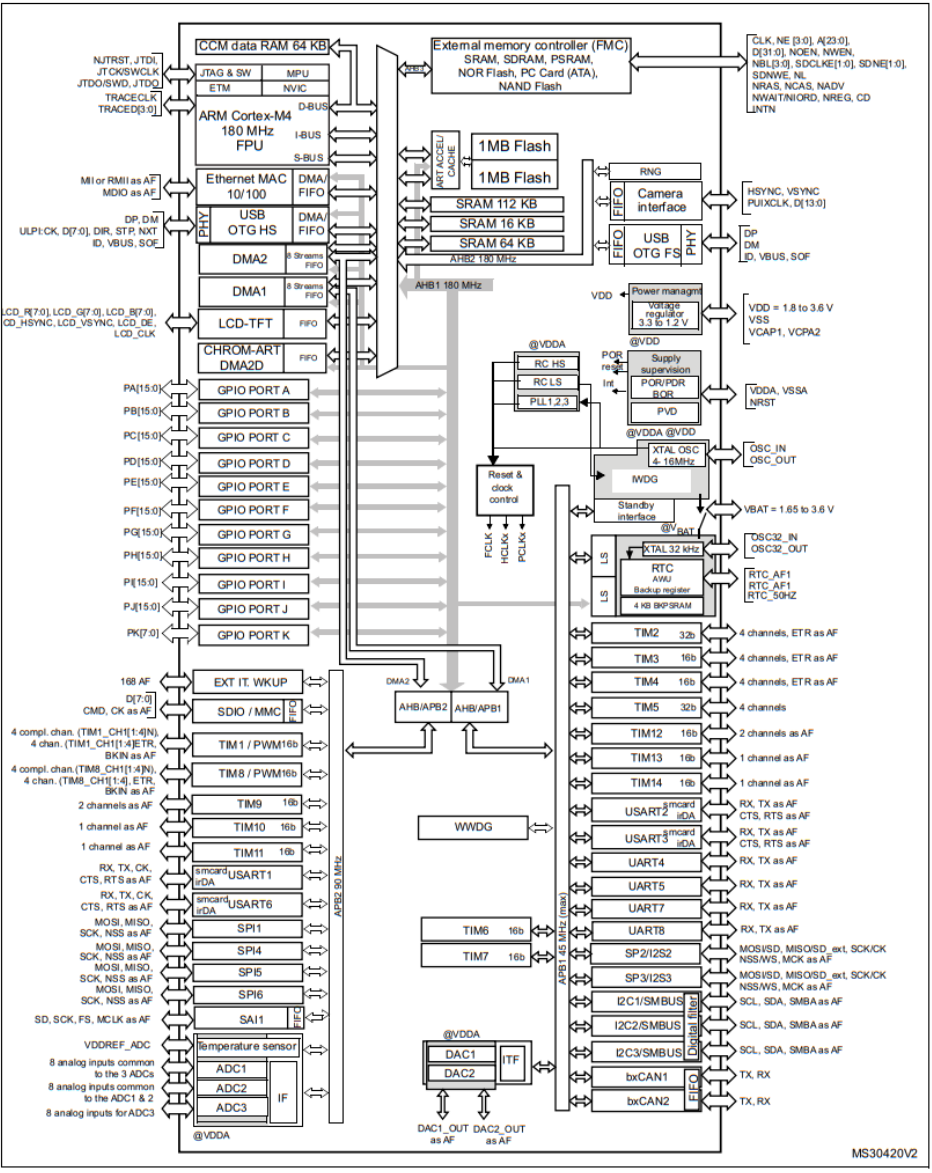
\includegraphics[width=14cm]{Imagenes/Diagrama_Bolques.png}
    \caption{Diagrama de bloques de la placa de desarrollo STM32F429ZIT6. Fuente y créditos: \cite{datasheet}.}
    \label{mcu-diagram}
\end{figure}


\subsubsection{Diagrama de pines}

En la figura \ref{Fig: Diagrama_pines1}, figura \ref{Fig: Diagrama_pines2} y figura \ref{Fig: Diagrama_pines3} se muestra el diagrama de pines del microcontrolador STM32F429 Discovery kit \cite{st-discovery-f429zi}. Para realizar este laboratorio se utilizaron los pines fueron el PA0, el cual es un convertidor analógico/digital, y el PA2, el cual se utilizó para habilitar la comunicación USART.


\begin{figure}[H]
\centering
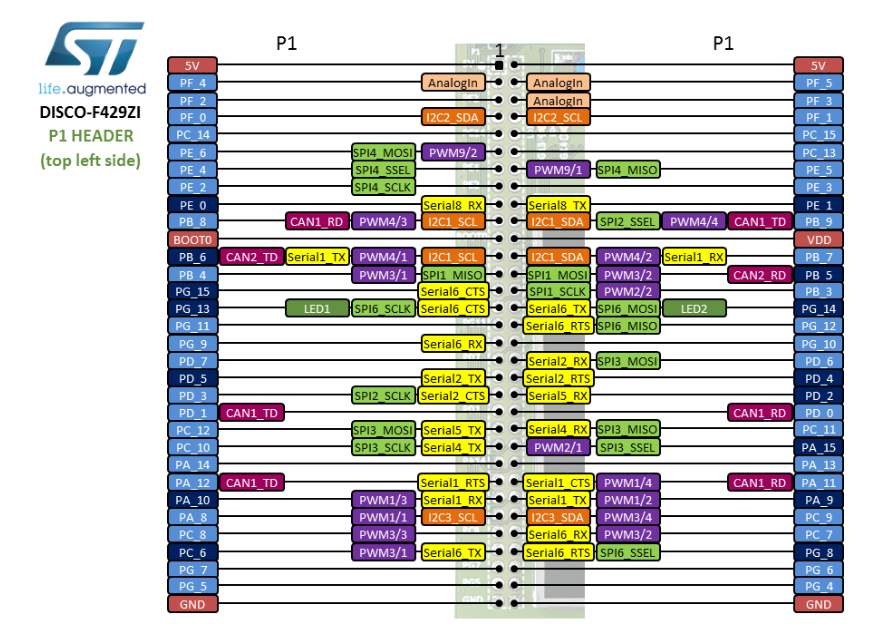
\includegraphics[width=0.8\textwidth]{Imagenes/Diagrama_Pines1.png} 
\caption{Diagrama de pines del STM32F429 Discovery kit parte 1. Fuente y créditos: \cite{st-discovery-f429zi}.}
\label{Fig: Diagrama_pines1}
\end{figure}

\begin{figure}[H]
\centering
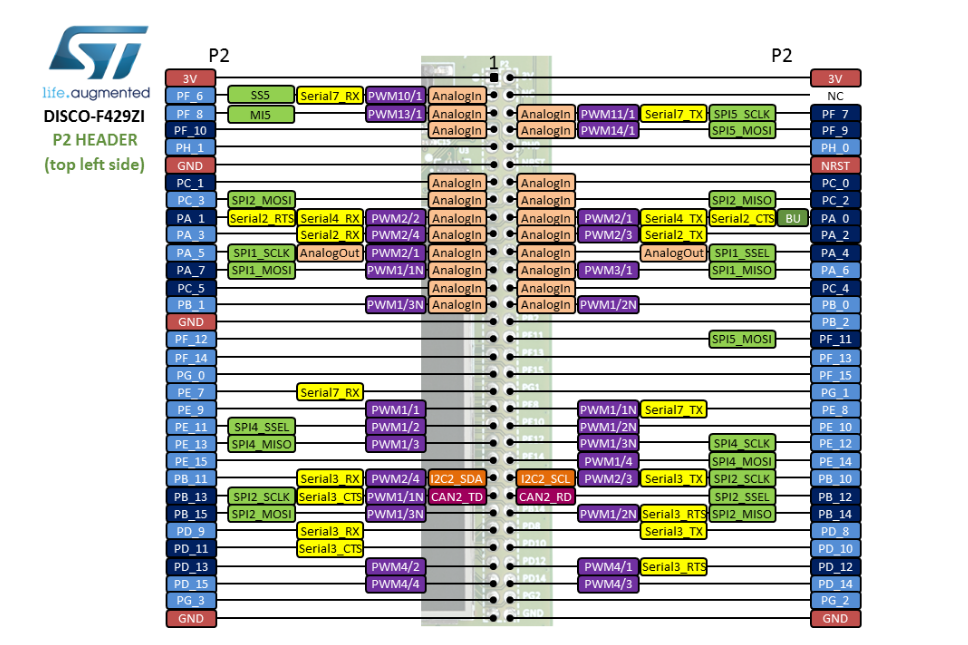
\includegraphics[width=0.8\textwidth]{Imagenes/Diagrama_Pines2.png} 
\caption{Diagrama de pines del STM32F429 Discovery kit parte 2. Fuente y créditos: \cite{st-discovery-f429zi}.}
\label{Fig: Diagrama_pines2}
\end{figure}

\begin{figure}[H]
\centering
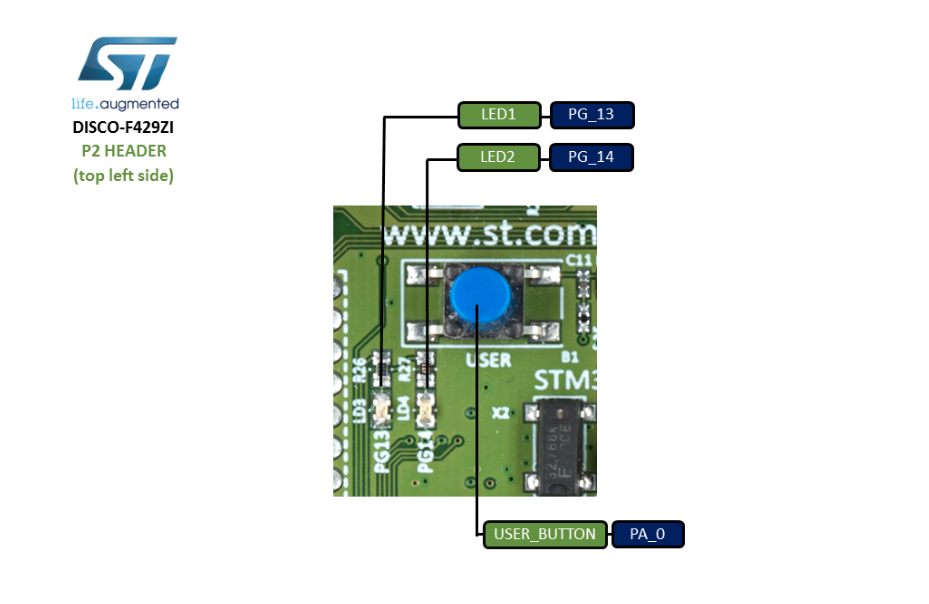
\includegraphics[width=0.8\textwidth]{Imagenes/Diagrama_Pines3.png} 
\caption{Diagrama de pines del STM32F429 Discovery kit parte 3. Fuente y créditos: \cite{st-discovery-f429zi}.}
\label{Fig: Diagrama_pines3}
\end{figure}

%\subsection{Registros utilizados}
%Muchos de los registros del ATMega328P son configurados automáticamente al encenderse el Arduino UNO \cite{datasheet, atmega}. De todos modos, los registros utilizados son \tt{MCUCR}, \tt{PORTx} y \tt{DDRx} con \tt{x = B, C, D} para configurar los pines como entrada o salida \& si es entrada, activar o desactivar las resistencias de \it{pull-up internas} \cite{ atmega}.
%Luego, se utilizan los registros \tt{SPCR}, \tt{SPSR} y \tt{SPDR} para configurar y activar la comunicación SPI. 
%Ahora, para acceder a los convertidores analógico-digital, se debe configurar los registros \tt{ADMUX}, \tt{ADCSRA}, \tt{ADCSRB}, \tt{ADCL} y \tt{ADCH} \cite{ atmega}.
%Finalmente, para utilizar USART, se configuran los registros \tt{UDRn}, \tt{UCSRnA}, \tt{UCSRnB}, \tt{UCSRnC}, \tt{UBRRnL} y \tt{UBRRnH} \cite{ atmega}.
%Nuevamente, la mayoría de los registros anteriores son automáticamente configurados. Los registros que deben ser configurados manualmente se acceden mediante funciones incorporados, no hace falta acceder directamente a dichos registros \cite{datasheet, atmega}.





\section{Diseño del hardware} 
Para el voltímetro se realizó una división tensiones \cite{electronics-stackexchange} como se observa en la figura \ref{hardware}, puesto que se necesita reducir el rango de tensiones al rango admitido por el Arduino UNO.


\begin{figure} [H]
    \centering
    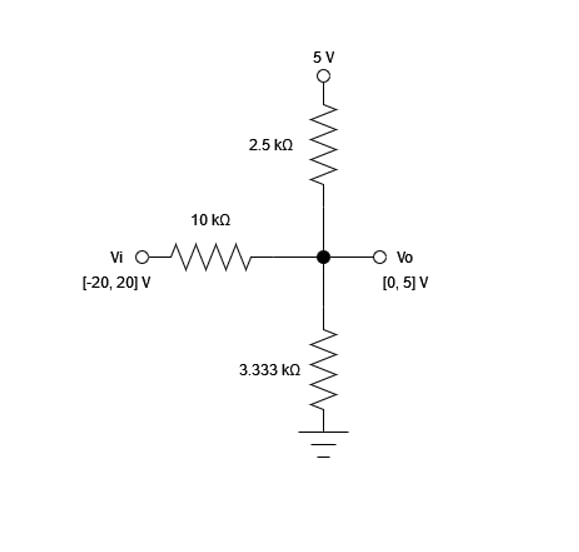
\includegraphics[width=11cm]{Imagenes/Hardware.jpg}
    \caption{Diseño de hardware para el voltímetro. Fuente y créditos: \cite{electronics-stackexchange}.}
    \label{hardware}
\end{figure}

Una vez que se realizó el diseño del divisor de tensiones, se realizó un diseño de un esquemático con la conexión de todos los componentes, y el circuitos anterior, como se muestra en la siguiente imagen.

\begin{figure} [H]
    \centering
    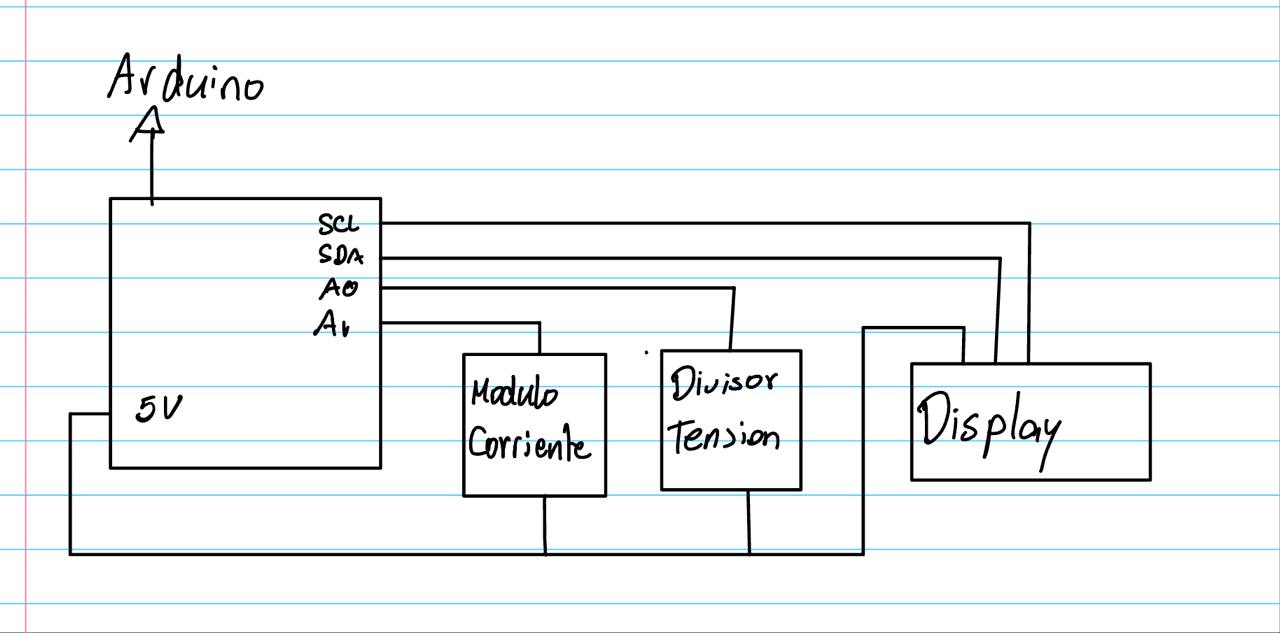
\includegraphics[width=11cm]{Imagenes/Esquematico.jpg}
    \caption{Esquemático del proyecto.}
    \label{Esquematico}
\end{figure}


\section{Diseño de los programas}
\subsection{Red neuronal}
Por un lado, se utilizó el \href{https://docs.edgeimpulse.com/docs/tutorials/end-to-end-tutorials/responding-to-your-voice}{tutorial} de Edge Impulse para crear y entrenar una red neuronal que detecte los comandos por voz. Los comandos son \tt{lumos}, \tt{musica} y \tt{tele}. Además, se siguió los pasos del mismo tutorial para flashear el modelo en el Arduino Nano BLE 33 Sense. Esto quiere decir que el código necesario para crear, entrenar y flashear al Arduino el modelo fue generado automáticamente por Edge Impulse, por lo que todos los créditos van hacia Edge Impulse \cite{tutorial}, los autores de este reporte de laboratorio solamente hicieron uso de los scripts generado por Edge Impulse.

\begin{figure}
    \centering
    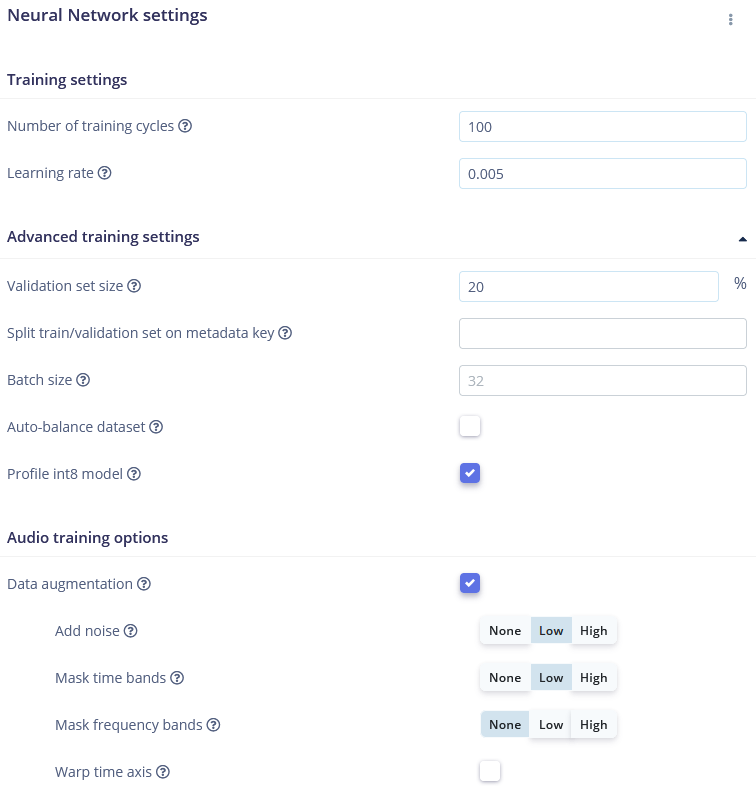
\includegraphics[width=12cm]{Imagenes/neural-1.png}
    \caption{Captura de pantalla de los parámetros de la red neuronal.}
    \label{neural-1}
\end{figure}

Además, los parámetros del modelo son las que Edge Impulse trae por defecto (figura \ref{neural-1}) así como recomendaciones que el tutorial menciona, cuya arquitectura de la red neuronal es el preset \tt{2D convolutional} (figura \ref{neural-2}) \cite{tutorial}. El código que se encarga de crear y entrenar la red se encuentra en el repositorio en la carpeta \tt{src/edge-impulse/} y el software necesario para flashear el modelo generado en el Arduino se encuentra en la carpeta \tt{src/firmware-arduino-nano-33-ble-sense/}.

\begin{figure}
    \centering
    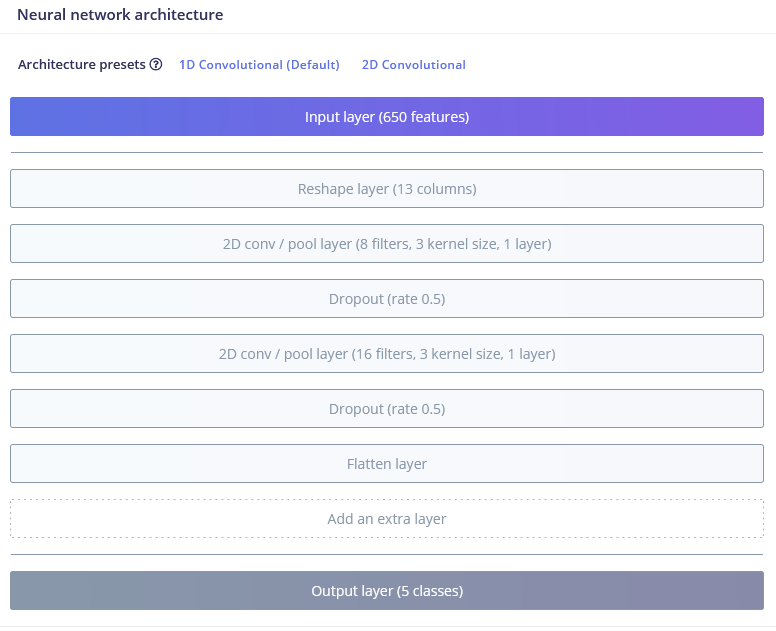
\includegraphics[width=12cm]{Imagenes/neural-2.png}
    \caption{Captura de pantalla de la arquitectura de la red neuronal.}
    \label{neural-2}
\end{figure}

\subsection{Diagrama de flujo del script de Python}
Por otro lado, se creó un script de Python (\tt{datos.py}) para poder recibir los datos del Arduino a la computadora. El diagrama de flujo se muestra en la figura \ref{py-diag}. La idea de este script es aprovechar que Edge Impulse tiene una interfaz en la terminal, esto es, tiene comandos para comunicarse con el Arduino. Tiene un comando denominado \tt{edge-impulse-run-impulse} que arroja en terminal las palabras, cuya cada palabra viene asociada un valor entre cero y uno. La palabra con el valor más alto es la palabra que el modelo cree lo que dijo el usuario \cite{edge-cli}.

\begin{figure}[th]
    \centering
    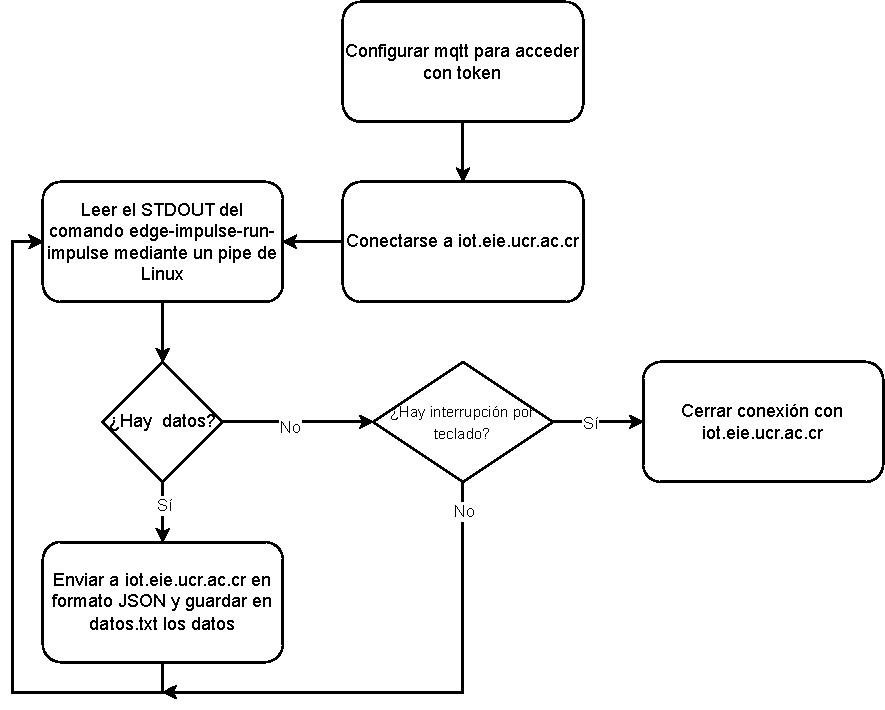
\includegraphics[width=13cm]{Imagenes/py.pdf}
    \caption{Diagrama de flujo del script para comunicar el Arduino con Thingsboard.}
    \label{py-diag}
\end{figure}

Ahora, mediante el pipe (\textbar) de Linux \cite{pipe} se puede redireccionar la salida del comando \tt{edge-impulse-run-impulse} a un script de Python en vez de arrojarlo en la terminal. Por lo tanto, lo que tendría que hacer el script de Python es recibir lo que \tt{edge-impulse-run-impulse} arroje y enviar a Thingsboard en formato JSON así como guardar en un archivo de texto las palabras con sus valores asociados. Por lo tanto, se debe correr \tt{edge-impulse-run-impulse --continuous | python3 datos.py} para poder recibir los datos del Arduino y guardalo en un archivo de texto así como enviarlo a Thingsboard. Sin embargo, el comando es largo y tedioso, así que el repositorio proporciona el script \tt{correr.sh} que ejecuta justamente ese comando para facilitar al usuario.
\section{Lista de equipos}
\begin{table}[H]
\centering
\resizebox{\textwidth}{!}{%
\begin{tabular}{|c|c|c|c|}
\hline
\textbf{Componente} & \textbf{Valor Nominal} & \textbf{Cantidad} & \textbf{Precio en el Mercado} \\ \hline
Arduino Nano BLE 33 Sense & - & 1 & \$40.50 \\ \hline
\end{tabular}%
}
\caption{Lista de Componentes \cite{nano33}.}
\label{tab:Lista_Componentes}
\end{table}
\section{Resultados y análisis}


\subsection{Verificación de los valores del giroscopio, batería y USART en la pantalla LCD}

Se realizaron pruebas por separado para poder verificar el correcto funcionamiento del giroscopio, de la batería y del USART.

\subsubsection{Verificación de la lectura del giroscopio}

    \begin{figure}[H]
        \begin{subfigure}{0.5\textwidth}
        \centering
        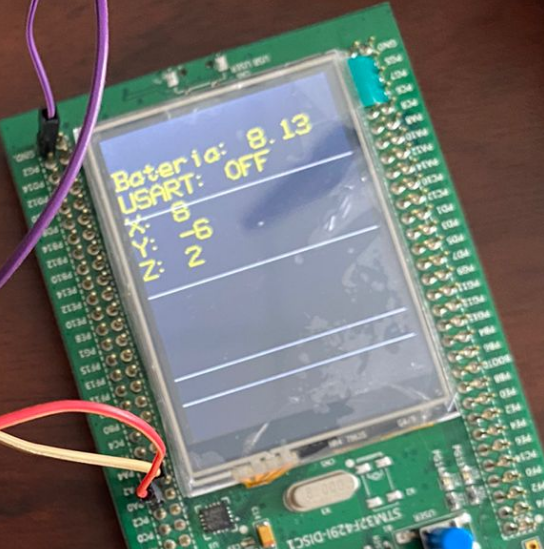
\includegraphics[width=\textwidth]{Imagenes/giroscopio2.png} 
        \caption{Prueba del giroscopio sobre la mesa sin movimiento.}
        \label{Fig:giroscopio}
    \end{subfigure}
    \begin{subfigure}{0.5\textwidth}
        \centering
        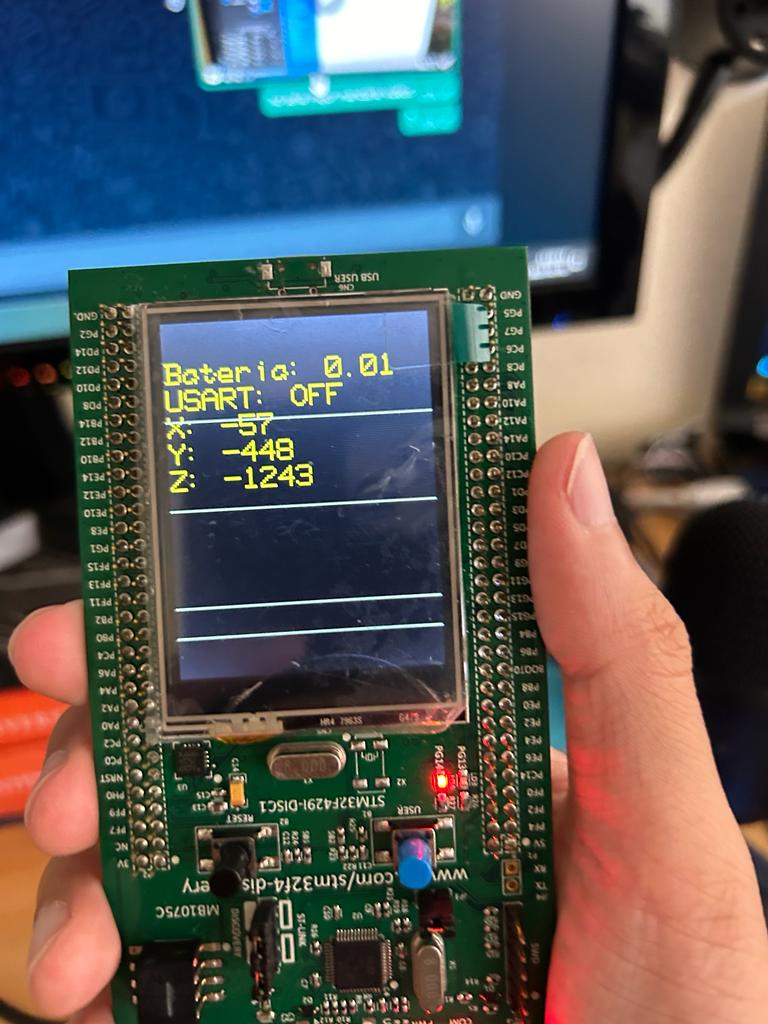
\includegraphics[width=\textwidth]{Imagenes/giroscopio.jpg} 
        \caption{Prueba del giroscopio levantándolo y con movimiento.}
        \label{Fig:giroscopio2}
    \end{subfigure}
    \end{figure}

En la figura \ref{Fig:giroscopio}, se puede observar que esta prueba fue cuando el microcontrolador estaba sobre la mesa, al estar en la mesa los valores que se obtienen son cercanos a 0, no son cero ya que es probable que el giroscopio sea muy sensible ante cualquier movimiento, aunque sea muy pequeño, por esta razón siempre marca algún valor aunque parezca que no esta en movimiento, y en la figura \ref{Fig:giroscopio2} se puede observar cómo la lectura del giroscopio cambia al someterse a un movimiento, en este caso se levantó de la mesa, demostrando así que los valores de \textit{X}, \textit{Y} y \textit{Z} cambian y así poder simular un sismógrafo.
Adicionalmente, en la entrega de este reporte se incluye tres videos, donde cualquiera de los tres videos se observa que se realiza la lectura del giroscopio correctamente.

\subsubsection{Verificación de la lectura de la Batería}

    \begin{figure}[H]
        \begin{subfigure}{0.5\textwidth}
        \centering
        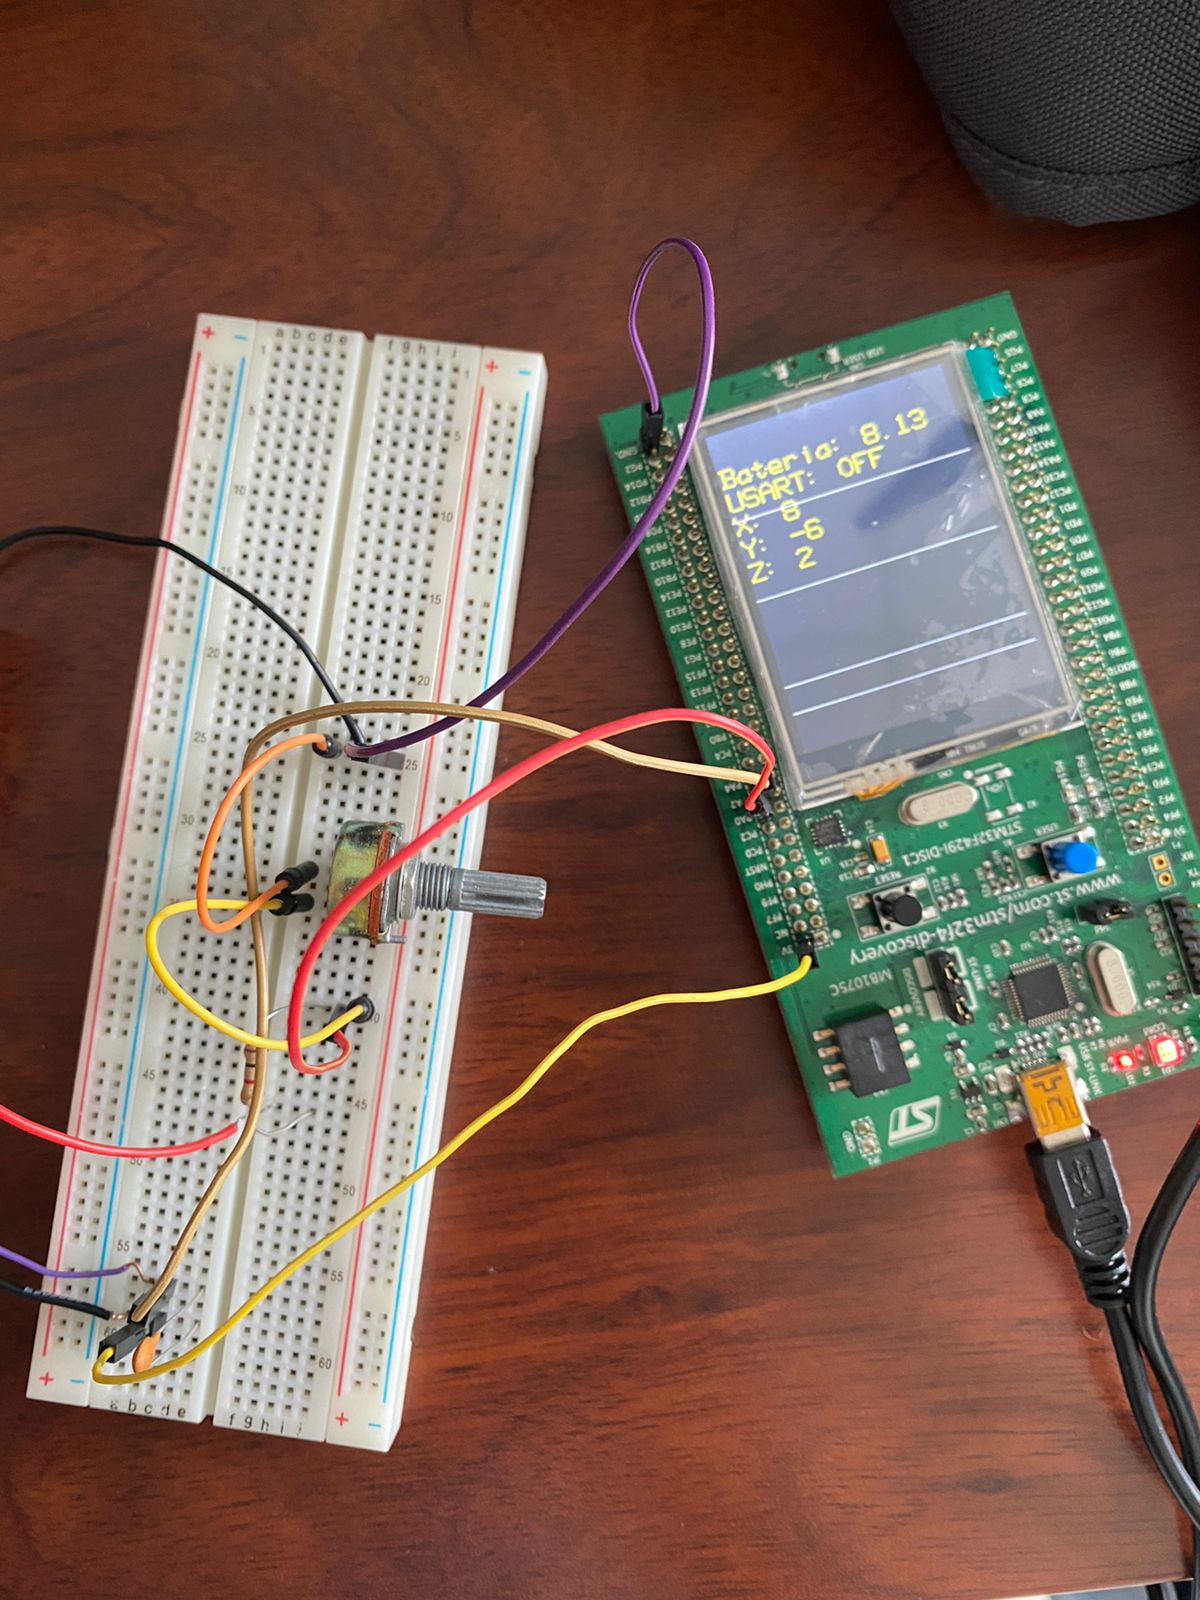
\includegraphics[width=\textwidth]{Imagenes/Prueba_Bat.jpg} 
        \caption{Prueba Batería en rango lejos de 7V.}
        \label{Fig:Prueba_Bat}
    \end{subfigure}
    \begin{subfigure}{0.5\textwidth}
        \centering
        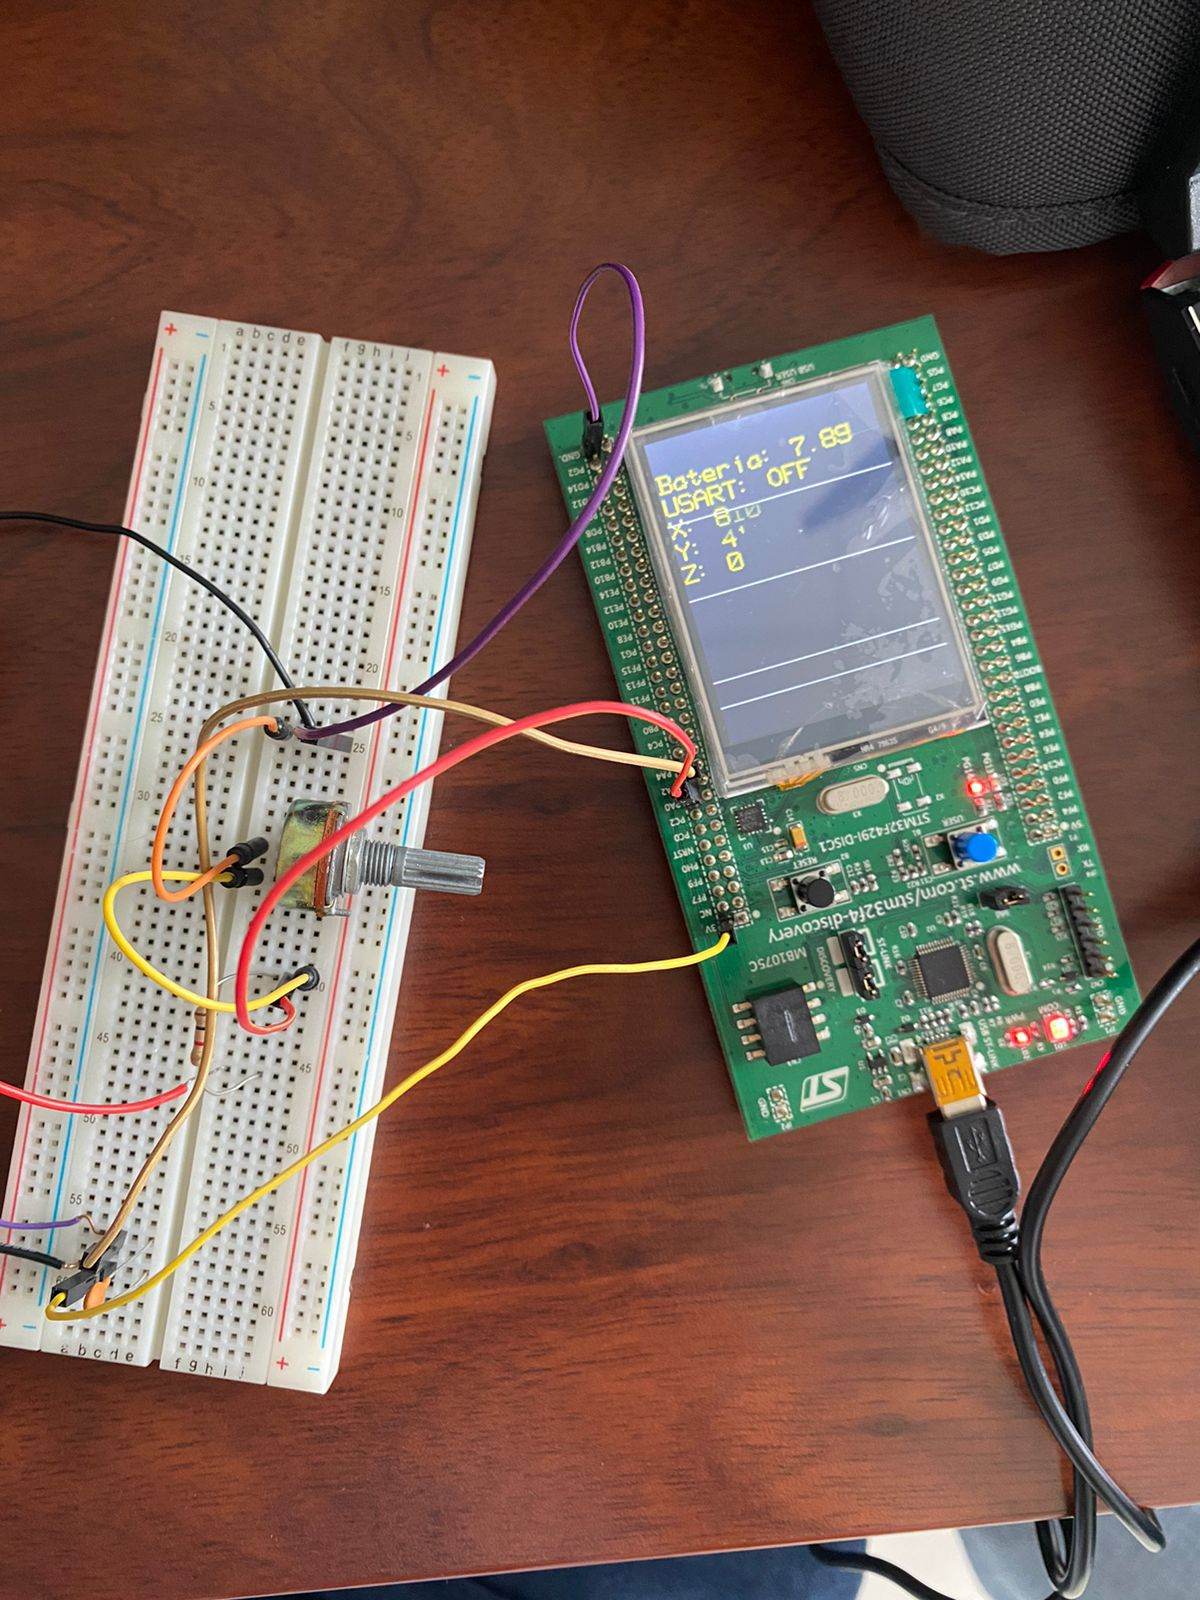
\includegraphics[width=\textwidth]{Imagenes/Prueba_Bat2.jpg} 
        \caption{Prueba Batería en rango cercano a 7V.}
        \label{Fig:Prueba_Bat2}
    \end{subfigure}
    \end{figure}

Como se observan en las figuras \ref{Fig:Prueba_Bat} y \ref{Fig:Prueba_Bat2}, se realizó una configuración de un divisor de tensiones con un potenciómetro con el fin de poder simular una caída de tensión de la batería, y conectando el pin PA0 a la salida de ese circuito y protegiendo así el STM32F429, entonces cuando el microcontrolador lee de la batería 8V o más, el cual se mantiene lejos del limite de operación del microcontrolador, el LED rojo que tiene incorporado el microcontrolador se encuentra apagado. Luego, se ajusta el potenciómetro de manera que lee una tensión por debajo de 8V y cerca a la tensión de operación, entonces el LED rojo se enciende y parpadea, indicando que se está trabajando con una tensión muy cercana a la tensión de operación del STM32F429 como se observa en la figura \ref{Fig:Prueba_Bat2}.


\subsubsection{Verificación de la lectura de la USART}

\begin{figure}[H]
    \begin{subfigure}{0.5\textwidth}
    \centering
    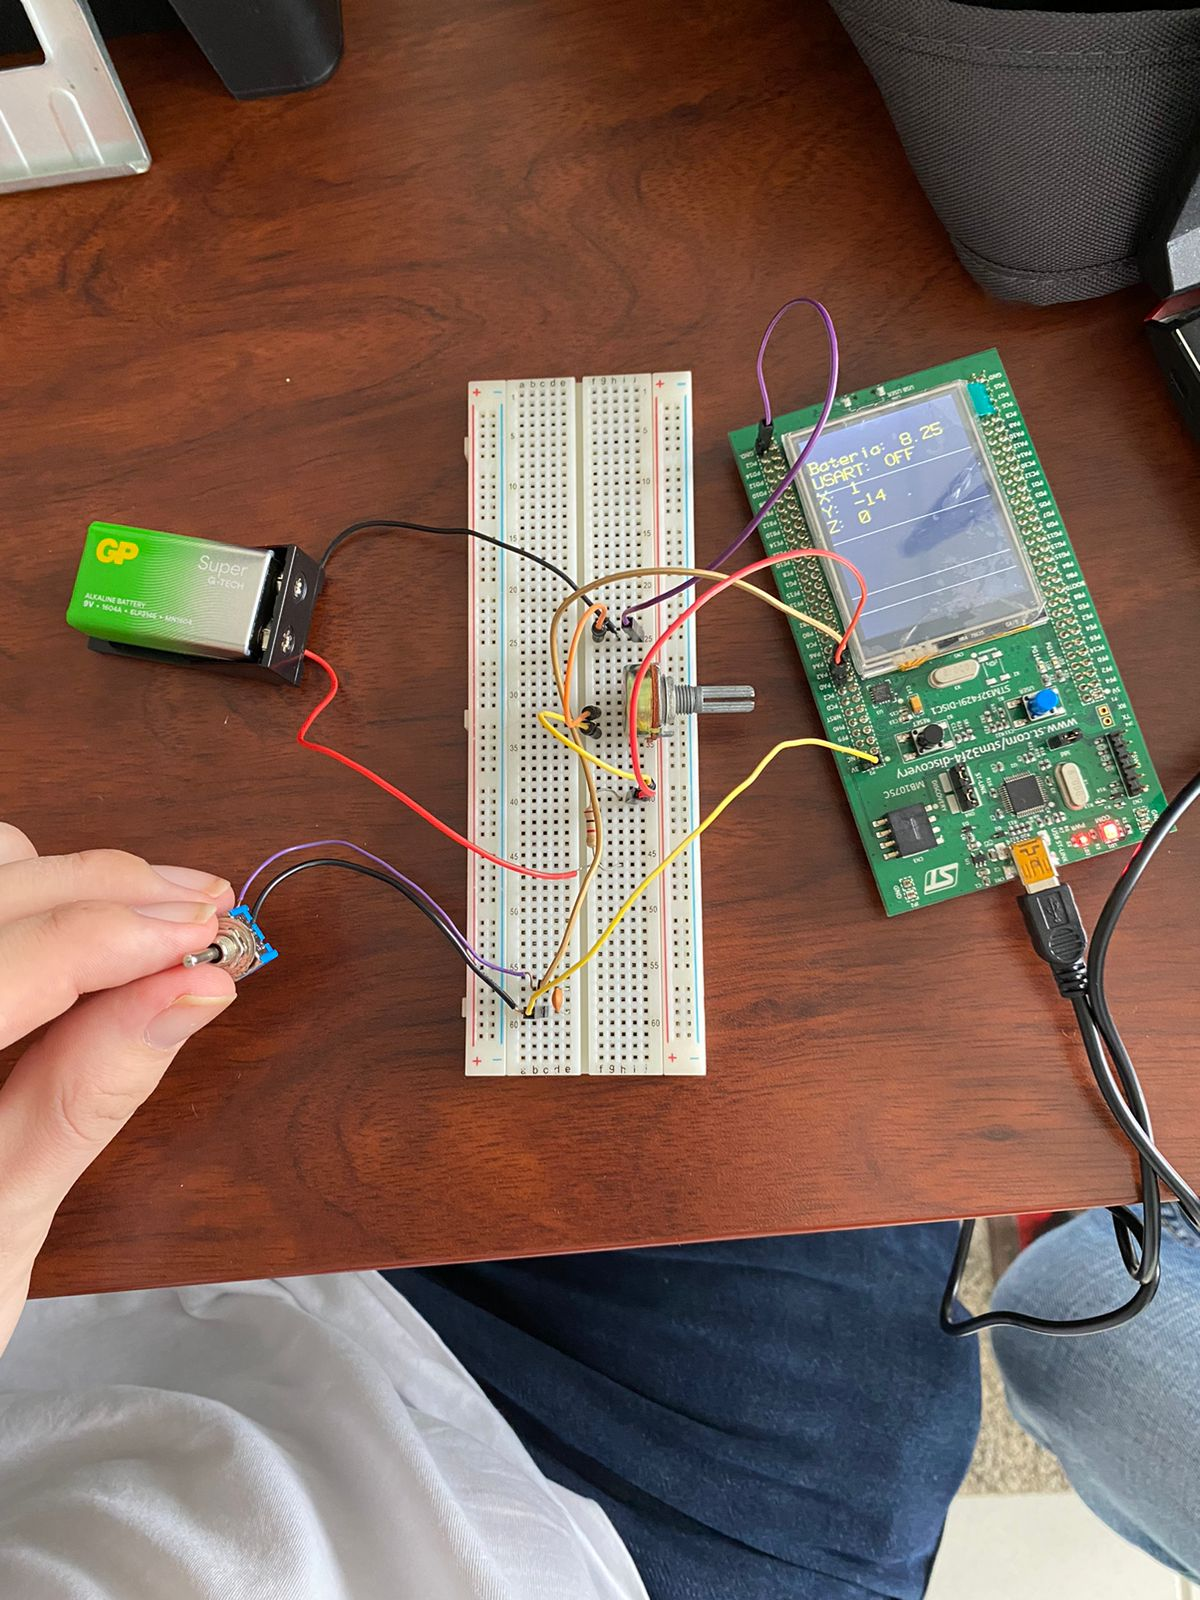
\includegraphics[width=\textwidth]{Imagenes/Prueba_USART.jpg} 
    \caption{Prueba USART en estado ``OFF''}
    \label{Fig:Prueba_USART}
\end{subfigure}
\begin{subfigure}{0.5\textwidth}
    \centering
    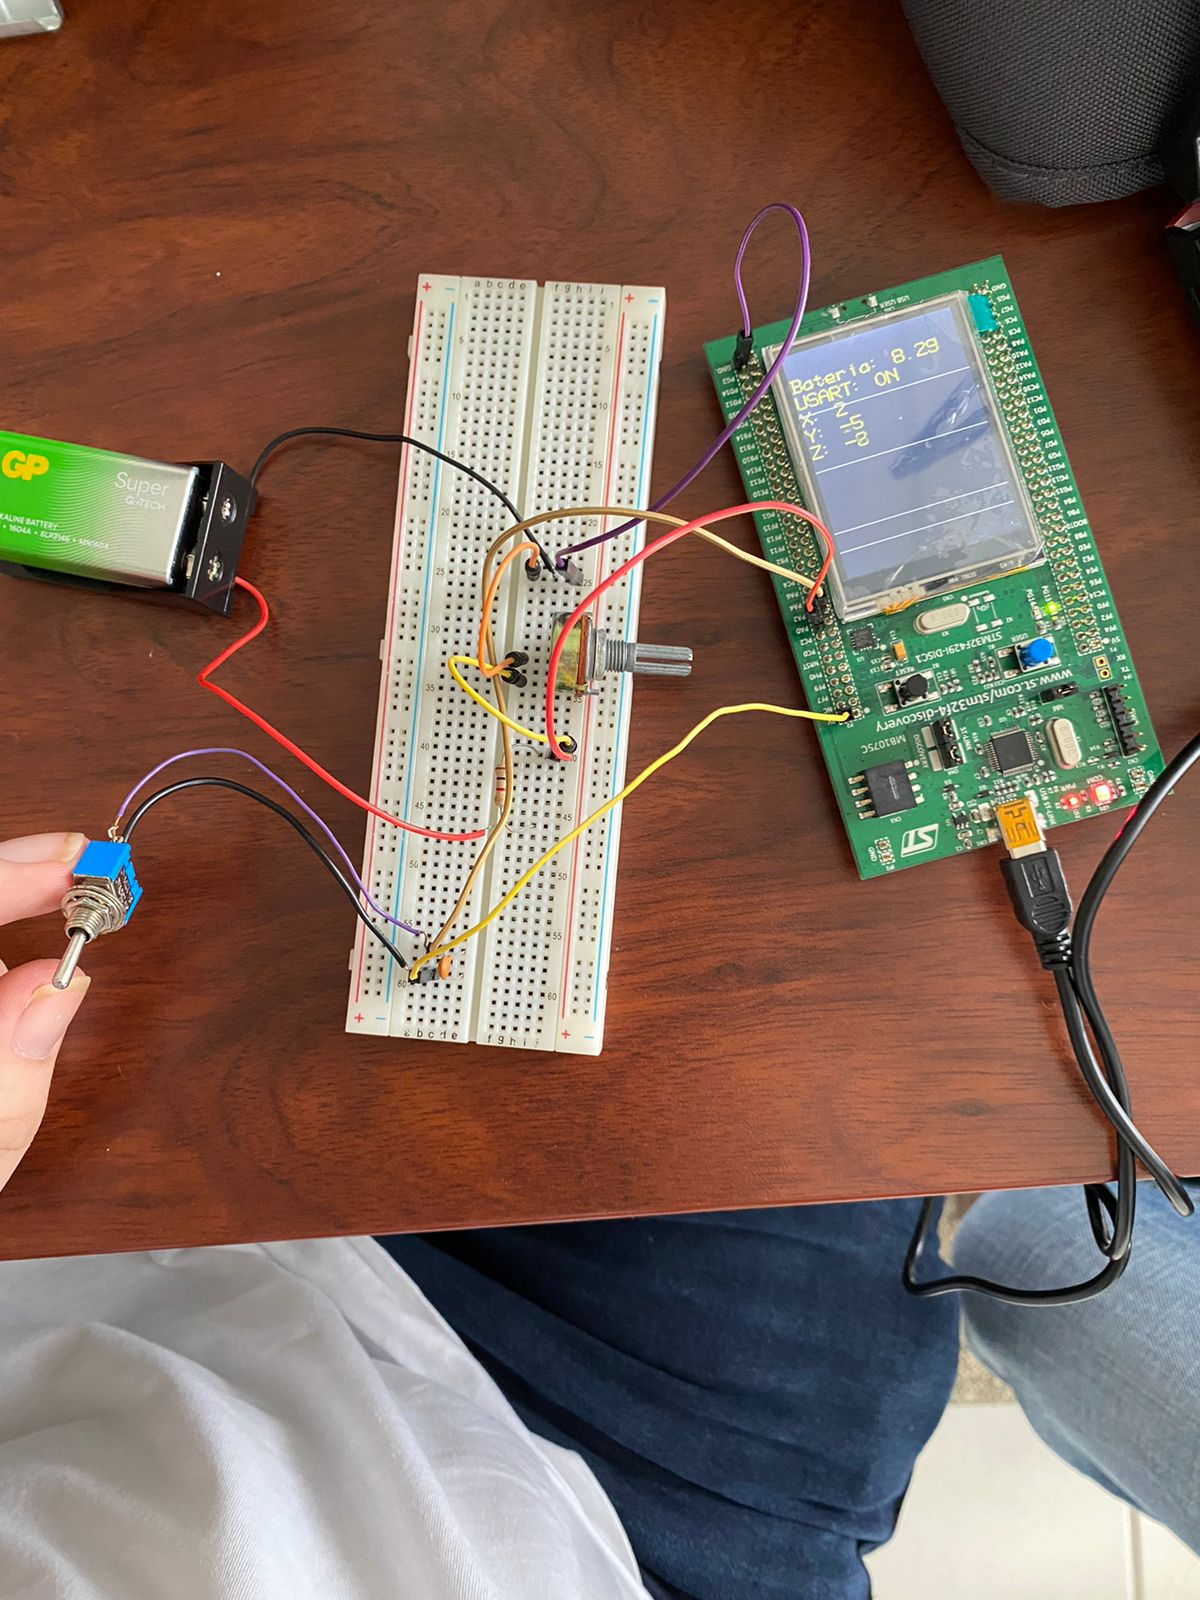
\includegraphics[width=\textwidth]{Imagenes/Prueba_USART2.jpg} 
    \caption{Prueba USART en estado ``ON''}
    \label{Fig:Prueba_USART2}
\end{subfigure}
\end{figure}

En las figuras \ref{Fig:Prueba_USART} y \ref{Fig:Prueba_USART2}, se observan las pruebas que se realizaron para verificar que cuando el switch se encuentra en ``OFF'', el microcontrolador lee que ese PIN esta en bajo, es decir, la comunicación USART esta desactiva como se observa en la pantalla LDC de la figura \ref{Fig:Prueba_USART}, cuando el switch esta en ``ON'', quiere decir que la el microcontrolador lee que el PIN se encuentra en alto y el LED verde del microcontrolador se enciende, es decir, que la comunicación USART se activa, como se observa en la pantalla LDC de la figura \ref{Fig:Prueba_USART2}. Para evitar el efecto rebote del switch, se le conectó un capacitor de 22 nF y no fue necesario conectarle una resistencia ya que este microcontrolador trae una resistencia interna según la hoja de datos \cite{stm32micro, datasheet}. 

\subsubsection{Verificación del funcionamiento de la Batería y el USART al mismo tiempo}

\begin{figure}[H]
    \begin{subfigure}{0.5\textwidth}
    \centering
    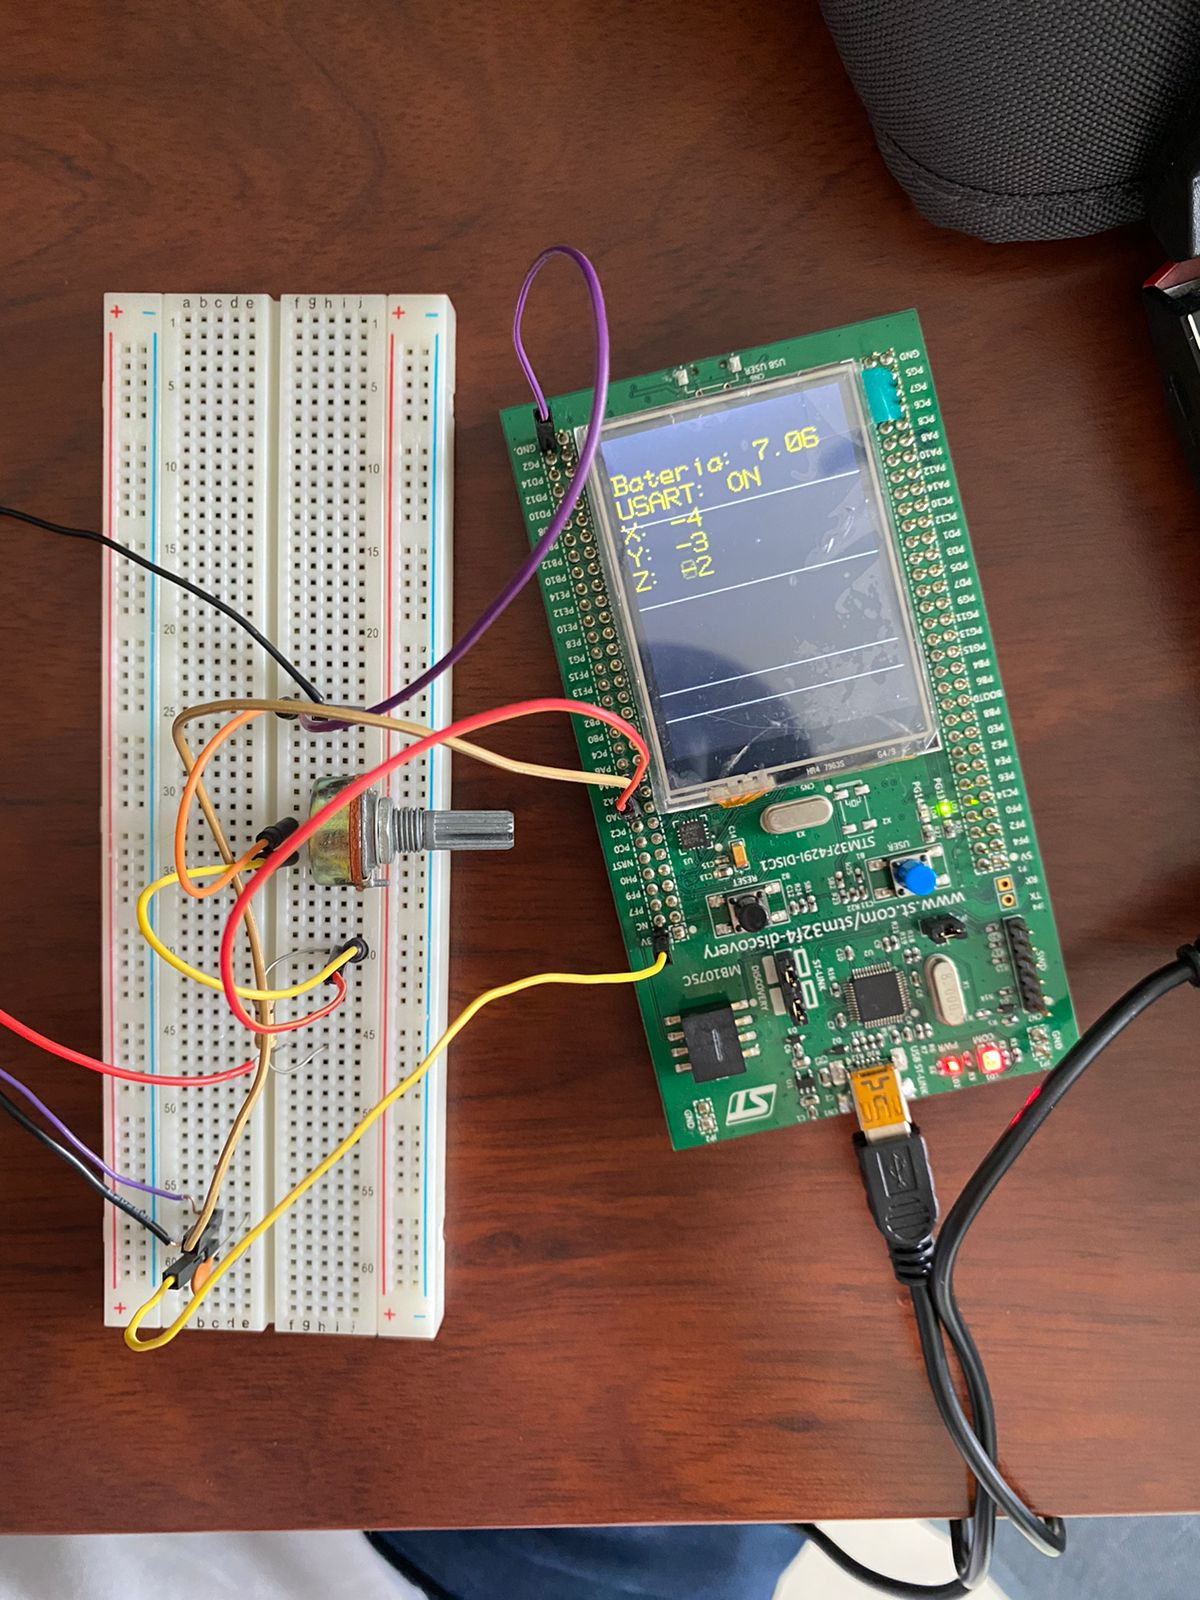
\includegraphics[width=0.9\textwidth]{Imagenes/Prueba_Bat_USART.jpg} 
    \caption{Prueba del funcionamiento de la USART y la Batería cercano a 7V.}
    \label{Fig:Prueba_Bat_USART}
\end{subfigure}
\begin{subfigure}{0.5\textwidth}
    \centering
    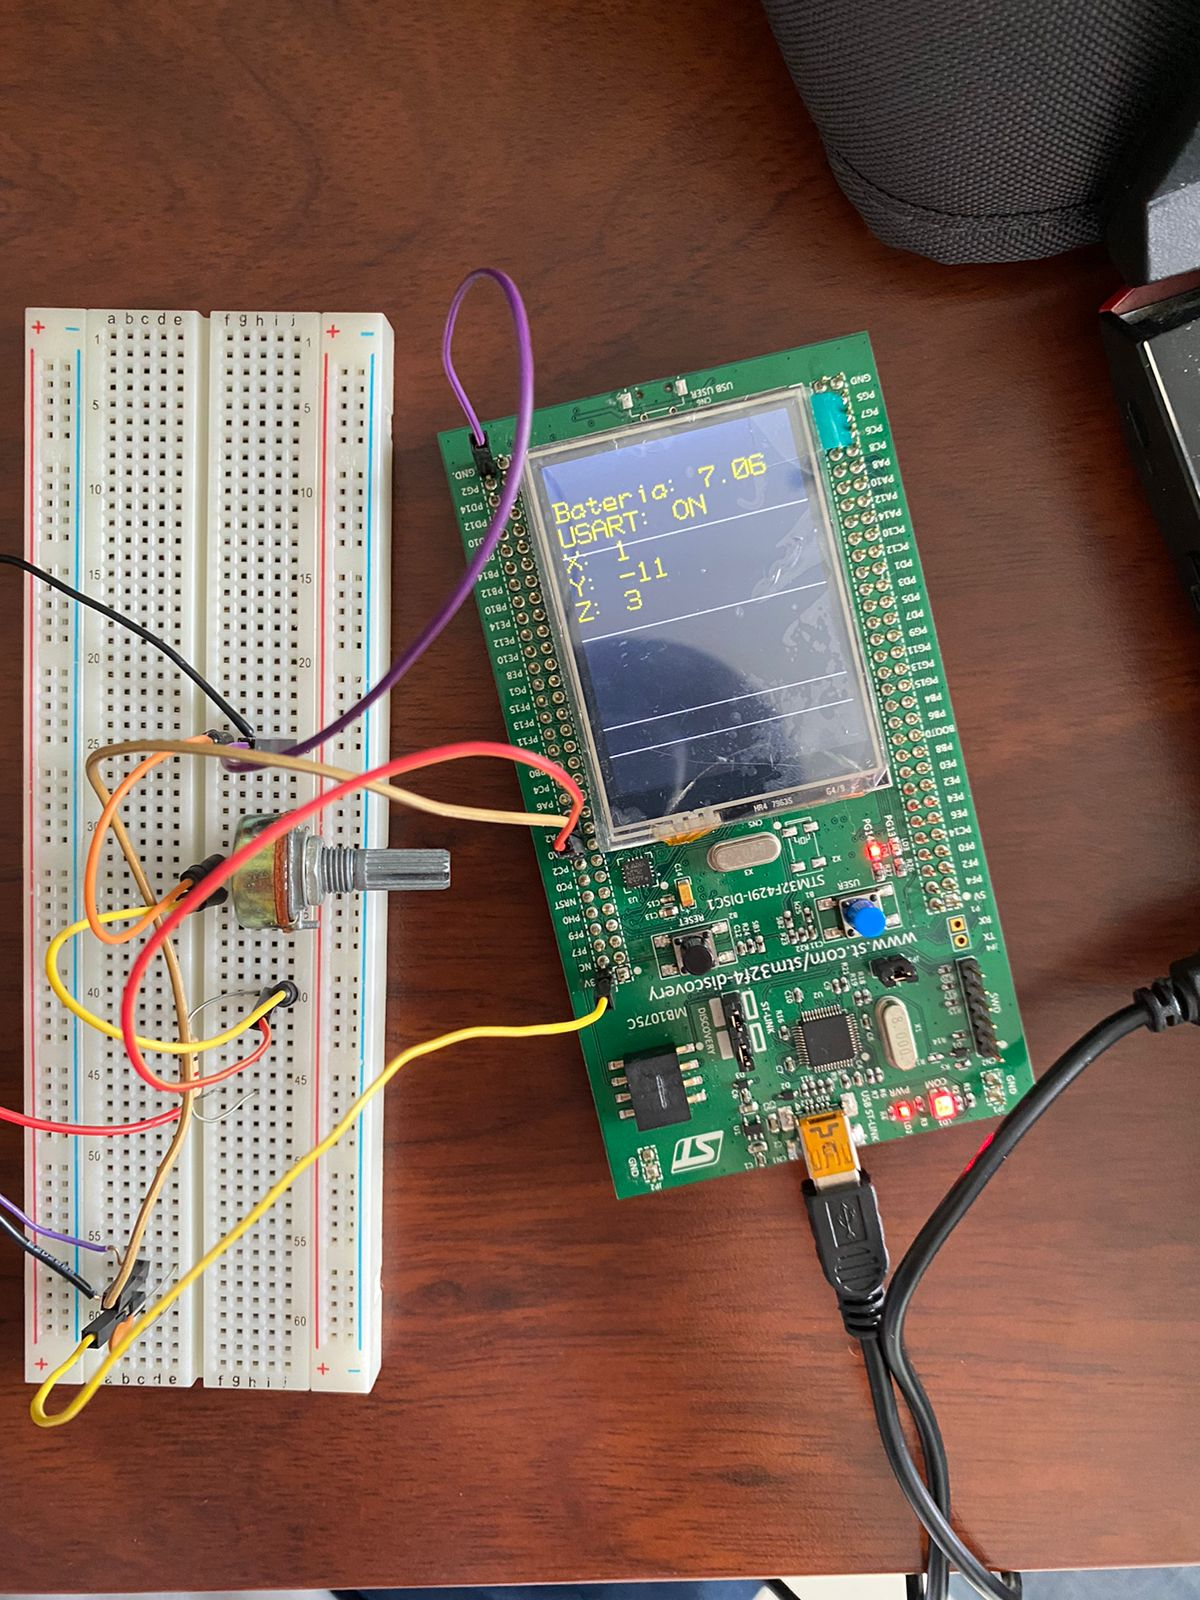
\includegraphics[width=\textwidth]{Imagenes/Prueba_Bat_USART2.jpg} 
    \caption{Prueba del funcionamiento de la USART y la Batería cercano a 7V.}
    \label{Fig:Prueba_Bat_USART2}
\end{subfigure}
\end{figure}

En las figuras \ref{Fig:Prueba_Bat_USART} y \ref{Fig:Prueba_Bat_USART2}, se observan como las 2 pruebas anteriores funcionan al mismo tiempo, cabe a destacar que las mangones que se muestran son únicamente cuando la tensión está cerca de la tensión de operación, es decir, esta cerca de los 7 V, de manera que el LED rojo se enciende y además se activa la comunicación USART, entonces los LED's parpadean de rojo a verde, comunicando que la comunicación USART esta activa y que la tensión de la batería esta cerca de la tensión de operación.



\subsection{Verificación que los datos se envíen correctamente por USART}
Ahora, se debe verificar que los datos se envíen correctamente por USART para ser mostrados en una terminal de la computadora. La figura \ref{usart-data-received} ilustra que sí se reciben los datos desde la placa de desarrollo y son mostrados correctamente en la terminal. En el video que se incluye en la entrega de este reporte, los videos \tt{demo\_usart\_off} ilustra que por más movimiento que se haga a la placa, éste no enviará los datos por USART ya que el USART está deshabilitado. En cambio, los videos \tt{demo\_usart\_iot\_on\_*} se muestra que cuando el USART está habilitado, los datos son enviados por comunicación serial y se reciben correctamente en la terminal.
\begin{figure}[H]
    \centering
    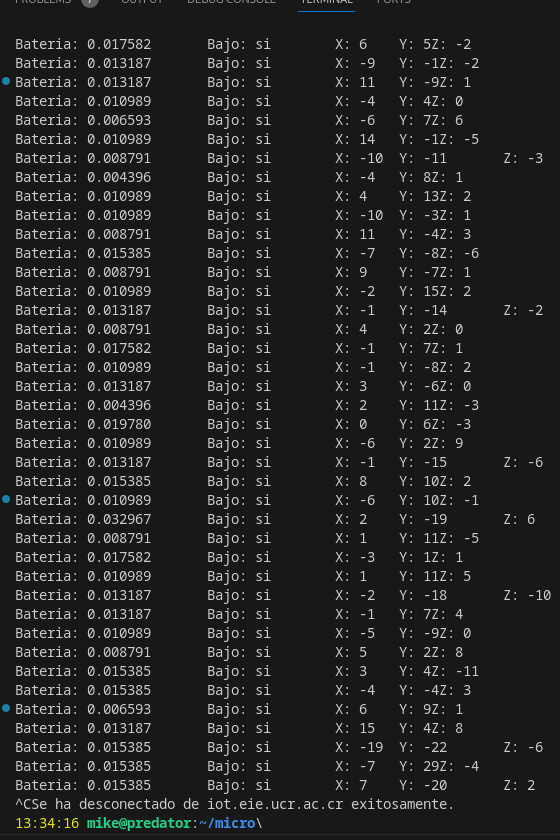
\includegraphics[width=12cm]{Imagenes/usart_data_received.png}
    \caption{Captura de pantalla de la terminal donde se reciben los datos por USART.}
    \label{usart-data-received}
\end{figure}

\subsection{Verificación de los datos se reflejen en iot.eie.ucr.ac.cr}
Luego, se debe comprobar que los datos recibidos por USART se envíen correctamente a \tt{iot.eie.ucr.ac.cr}. La figura \ref{iot-data-received} ilustra que los datos son enviados correctamente a Thingsboard y se muestran correctamente en el dashboard. Los videos \tt{demo\_usart\_iot\_on\_*} incluidos en la entrega ilustran que efectivamente los datos llegan correctamente a Thingsboard puesto que la página web se actualiza cuando se envía datos desde la placa de desarrollo.
\begin{figure}[H]
    \centering
    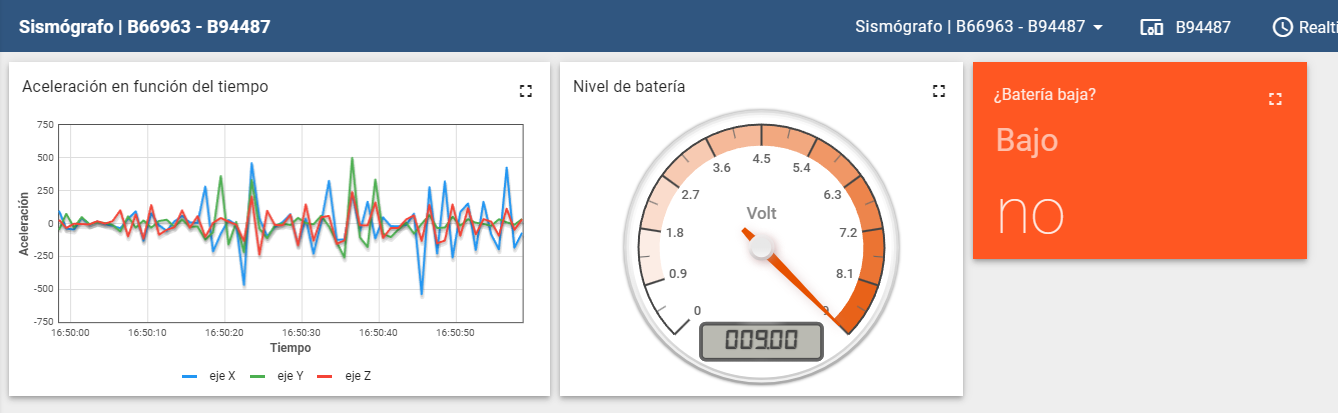
\includegraphics[width=\textwidth]{Imagenes/iot_data_received.png}
    \caption{Captura de pantalla de la terminal donde se envían a \tt{iot.eie.ucr.ac.cr} los datos.}
    \label{iot-data-received}
\end{figure}


\subsection{Verificación de las tensiones se encuentren dentro del rango seguro}

Con ayuda de un voltímetro se verificó que las tensiones que lee el microcontrolador se encuentran en rango seguro según la hoja del fabricante, y así evitar que se queme algún componente del microcontrolador \cite{stm32micro, datasheet}.


\begin{figure}[H]
    \begin{subfigure}{0.5\textwidth}
    \centering
    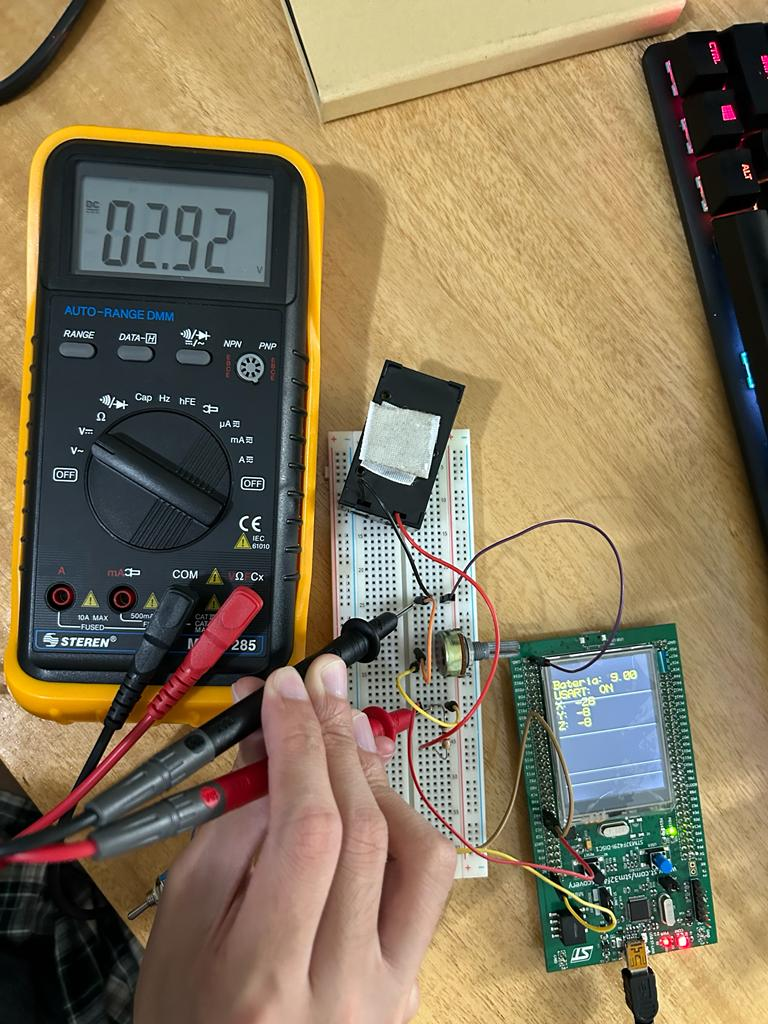
\includegraphics[width=\textwidth]{Imagenes/BATERIA.jpg} 
    \caption{Lectura de la tensión que lee del PIN PA0 (la batería) el microcontrolador}
    \label{Fig:BATERIA}
\end{subfigure}
\begin{subfigure}{0.5\textwidth}
    \centering
    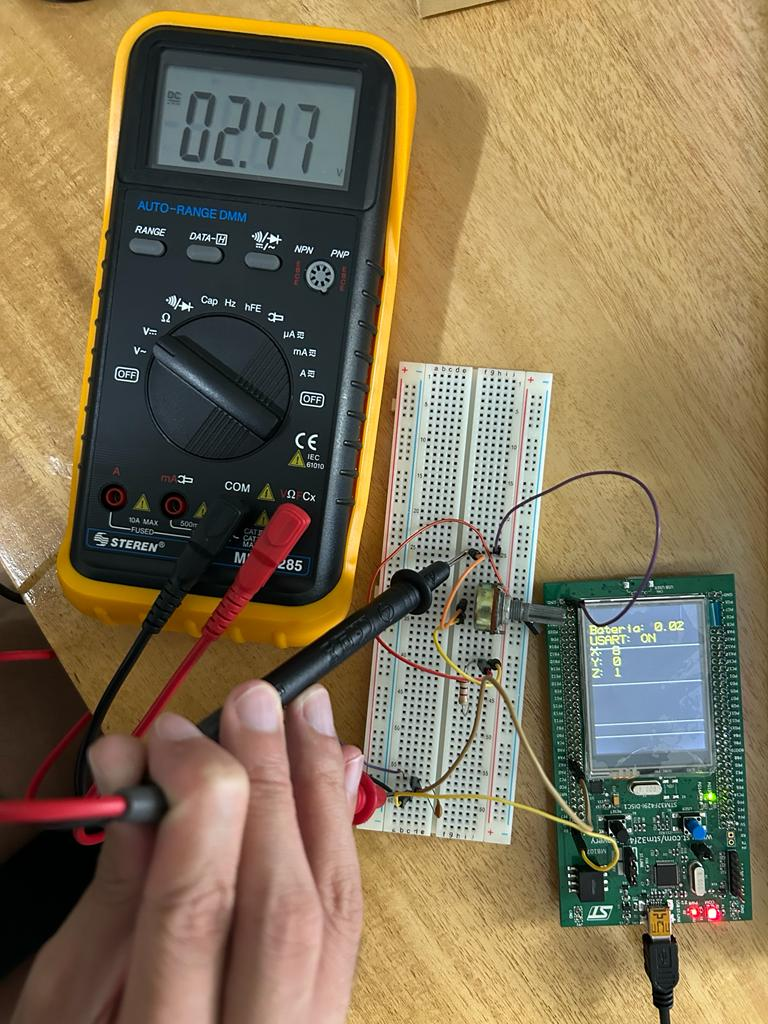
\includegraphics[width=\textwidth]{Imagenes/USART.jpg} 
    \caption{Lectura de la tensión que lee del PIN PA2 el microcontrolador}
    \label{Fig:USART}
\end{subfigure}
\end{figure}

Como se puede ver, en las figuras \ref{Fig:BATERIA} y \ref{Fig:USART} se observa que el voltaje que marca son 2.92V para la etapa de la batería y para la etapa del switch que controla el USART marca 2.47V, según la hoja del fabricante el valor máximo de tensión que soporta los pines es 4 V según la hoja del fabricante \cite{stm32micro, datasheet}, y ambos valores están por debajo de esa de esa tensión, por lo tanto se concluye que se está trabajando con unas tensiones seguras para el microcontrolador y así no dañar el STM32F429.





































\section{Conclusiones y recomendaciones}
\begin{itemize}
    \item El laboratorio se concluyó de manera satisfactoria ya que se cumplió con todas las especificaciones del enunciado.
    \item Esto incluye la conversión correcta del rango de tensiones $[\SI{-24}{\volt}, \SI{24}{\volt}]$ a $[\SI{0}{\volt}, \SI{5}{\volt}]$, la implementación del \it{switch} para medir en AC o DC y mostrar correctamente las lecturas en la pantalla LCD.
    \item Además, se pudo implementar el envío de las lecturas por comunicación serial para ser recibidos por un script de Python que guarda las lecturas en un archivo csv.
    \item Los cuatro canales de tensión son totalmente independientes uno del otro.
    \item Se puede observar que las tensiones no poseen riesgo de quemar algún componente, en especial el Arduino UNO, ya que los valores están dentro del rango de operación segura.
\end{itemize}



 






\newpage


\bibliographystyle{IEEEtranS}
\bibliography{bibliografia.bib}
\newpage

\newpage

\section{Anexos}
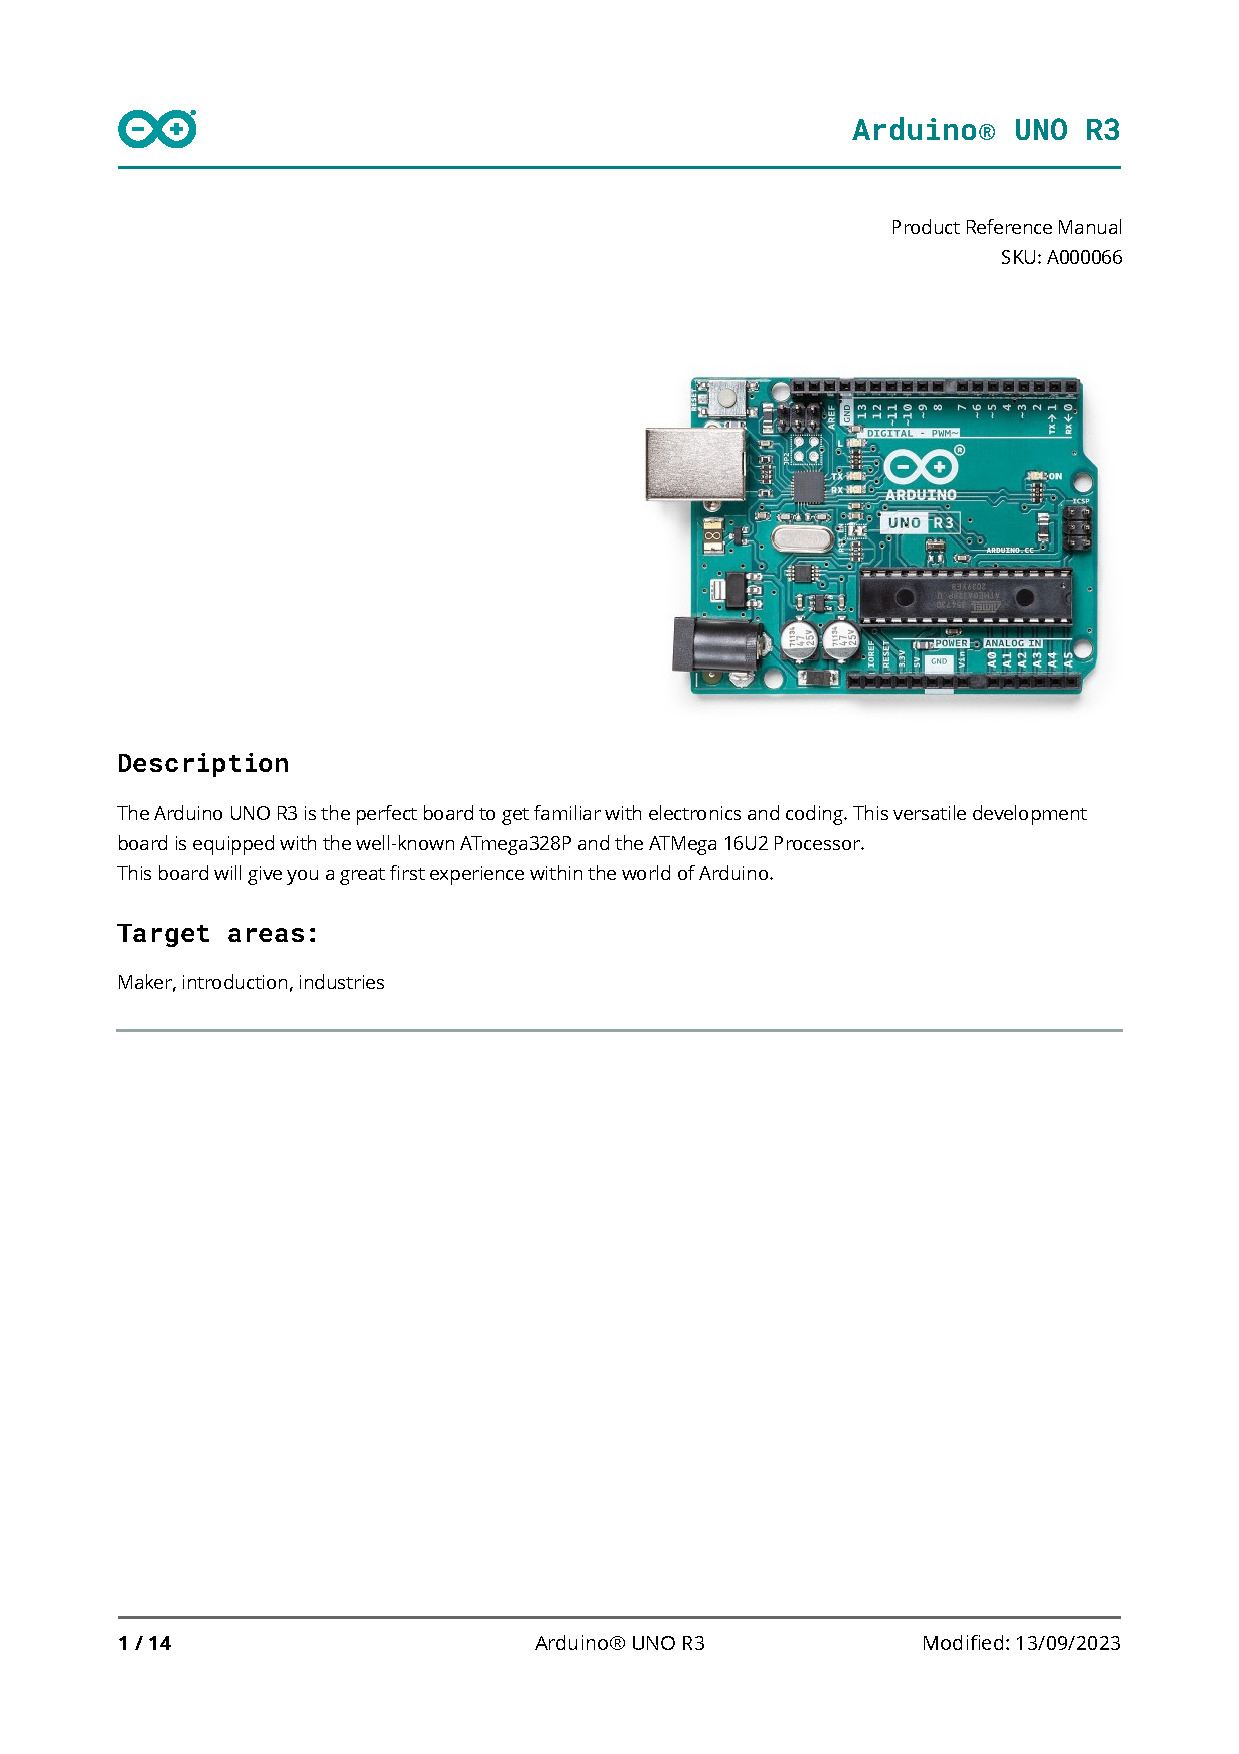
\includepdf[pages={1-10}]{Documentos/Arduino.pdf}
\includepdf[pages={1-6,58-59, 72-73, 135-136, 140-142, 143-144, 159-162, 205-207, 217-220}]{Documentos/ATMega328P.pdf}
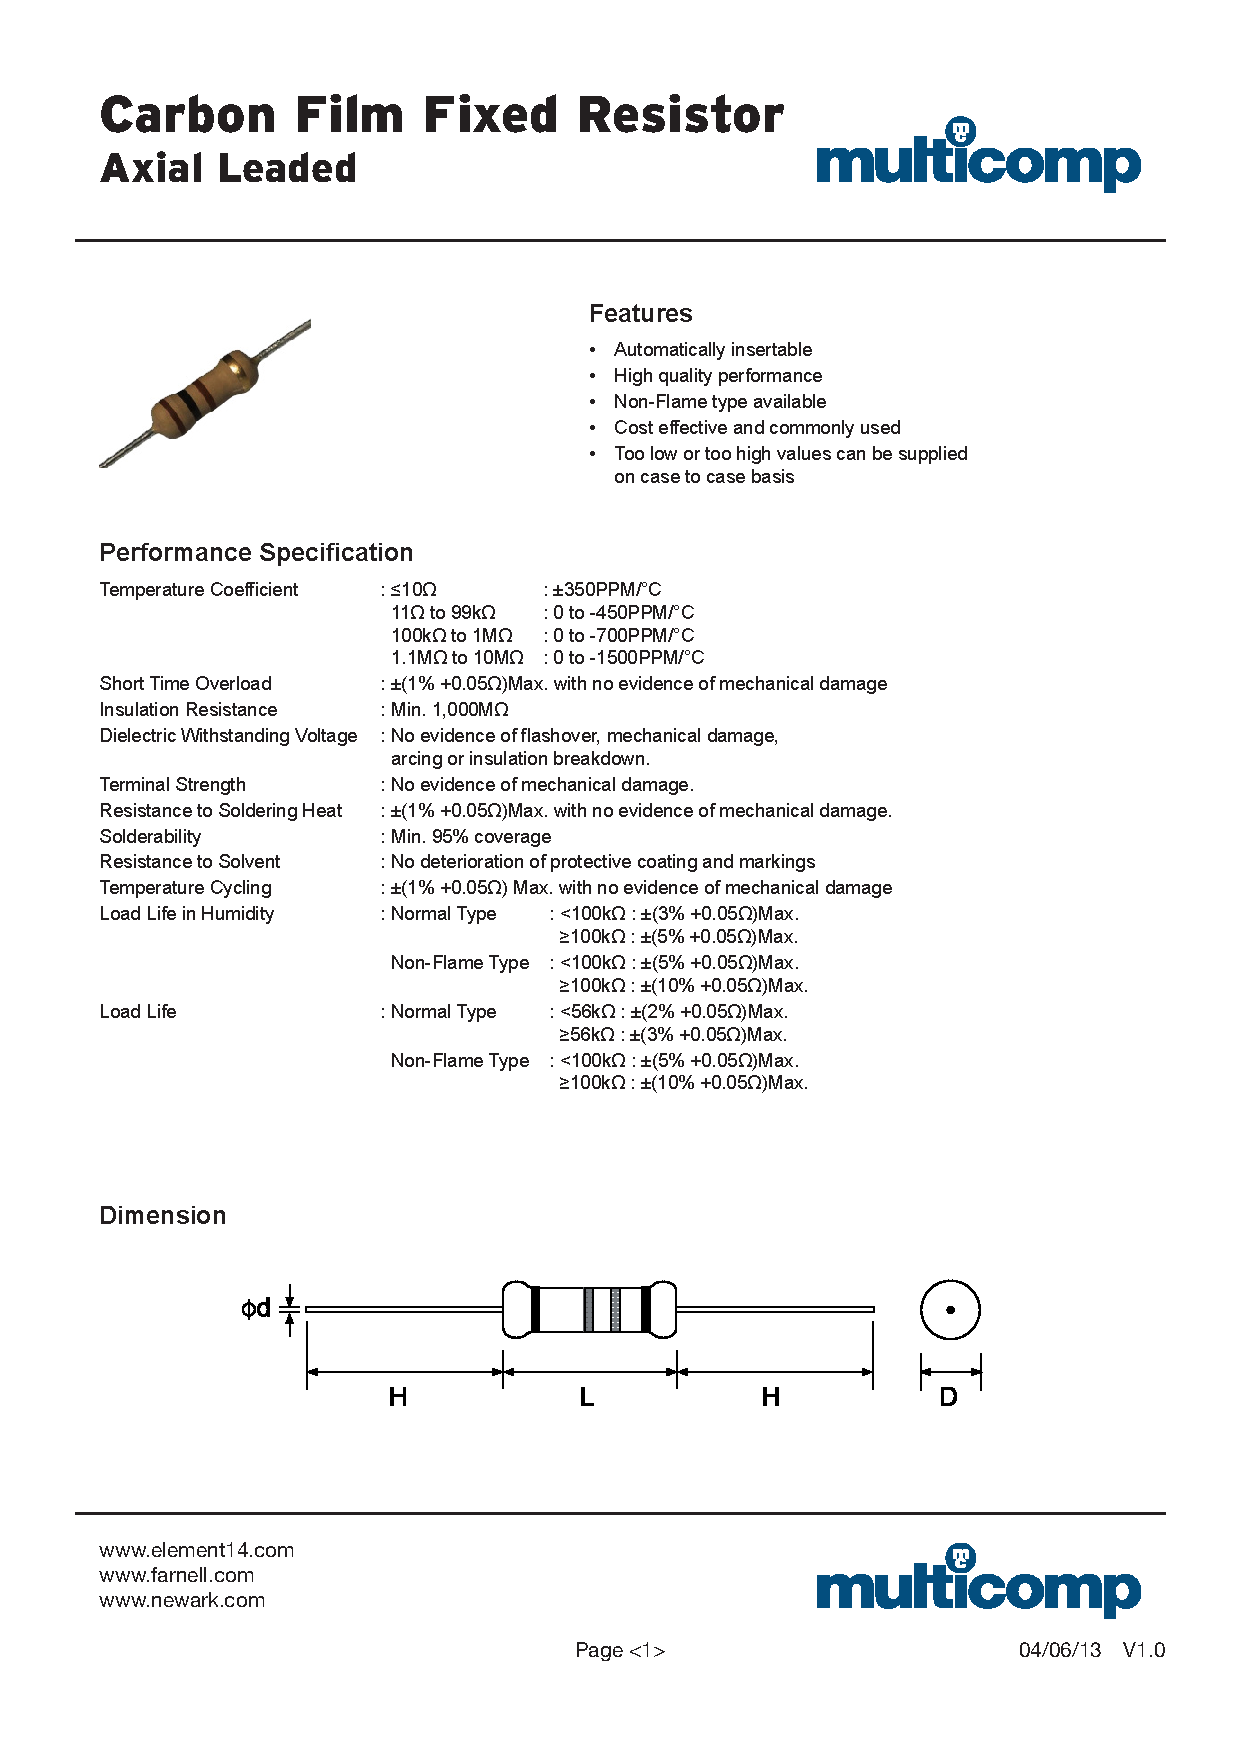
\includepdf[pages={1-2}]{Documentos/resistor.pdf}
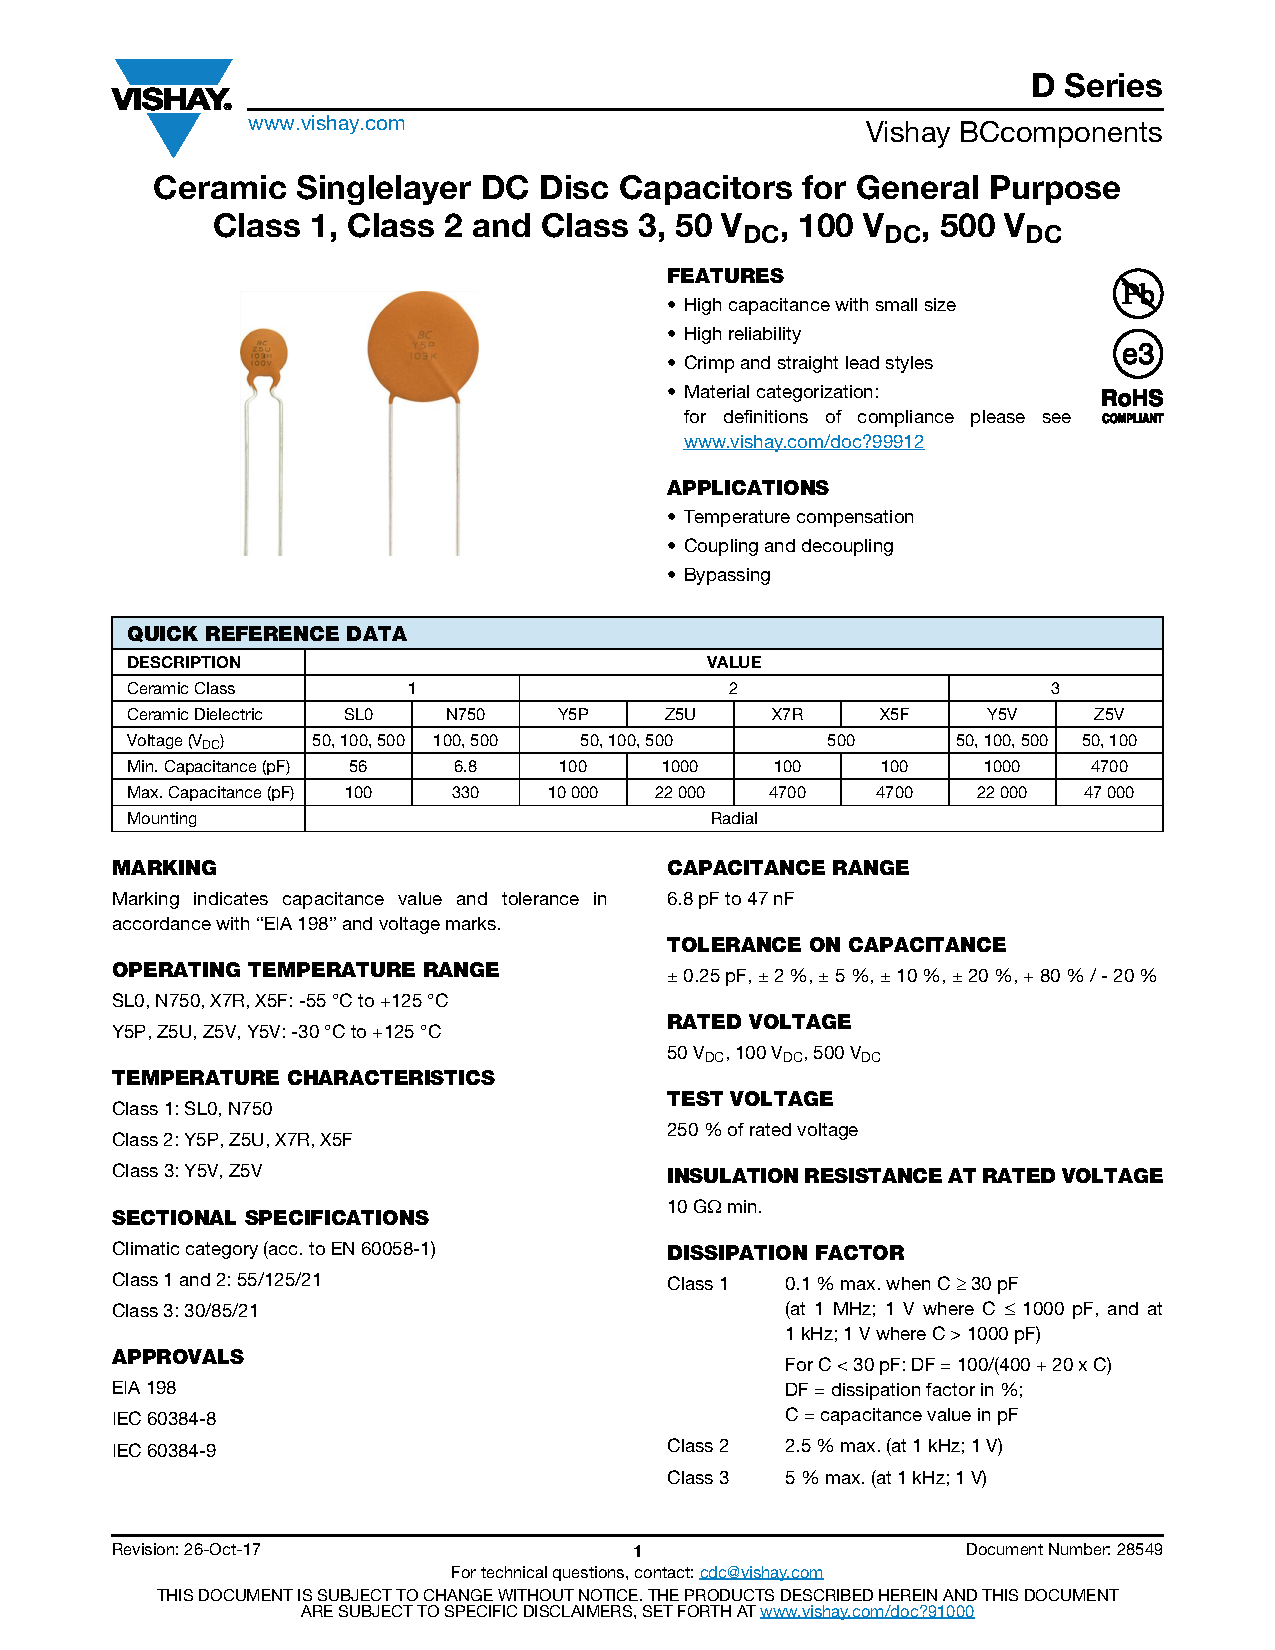
\includepdf[pages={1}]{Documentos/capacitor.pdf}
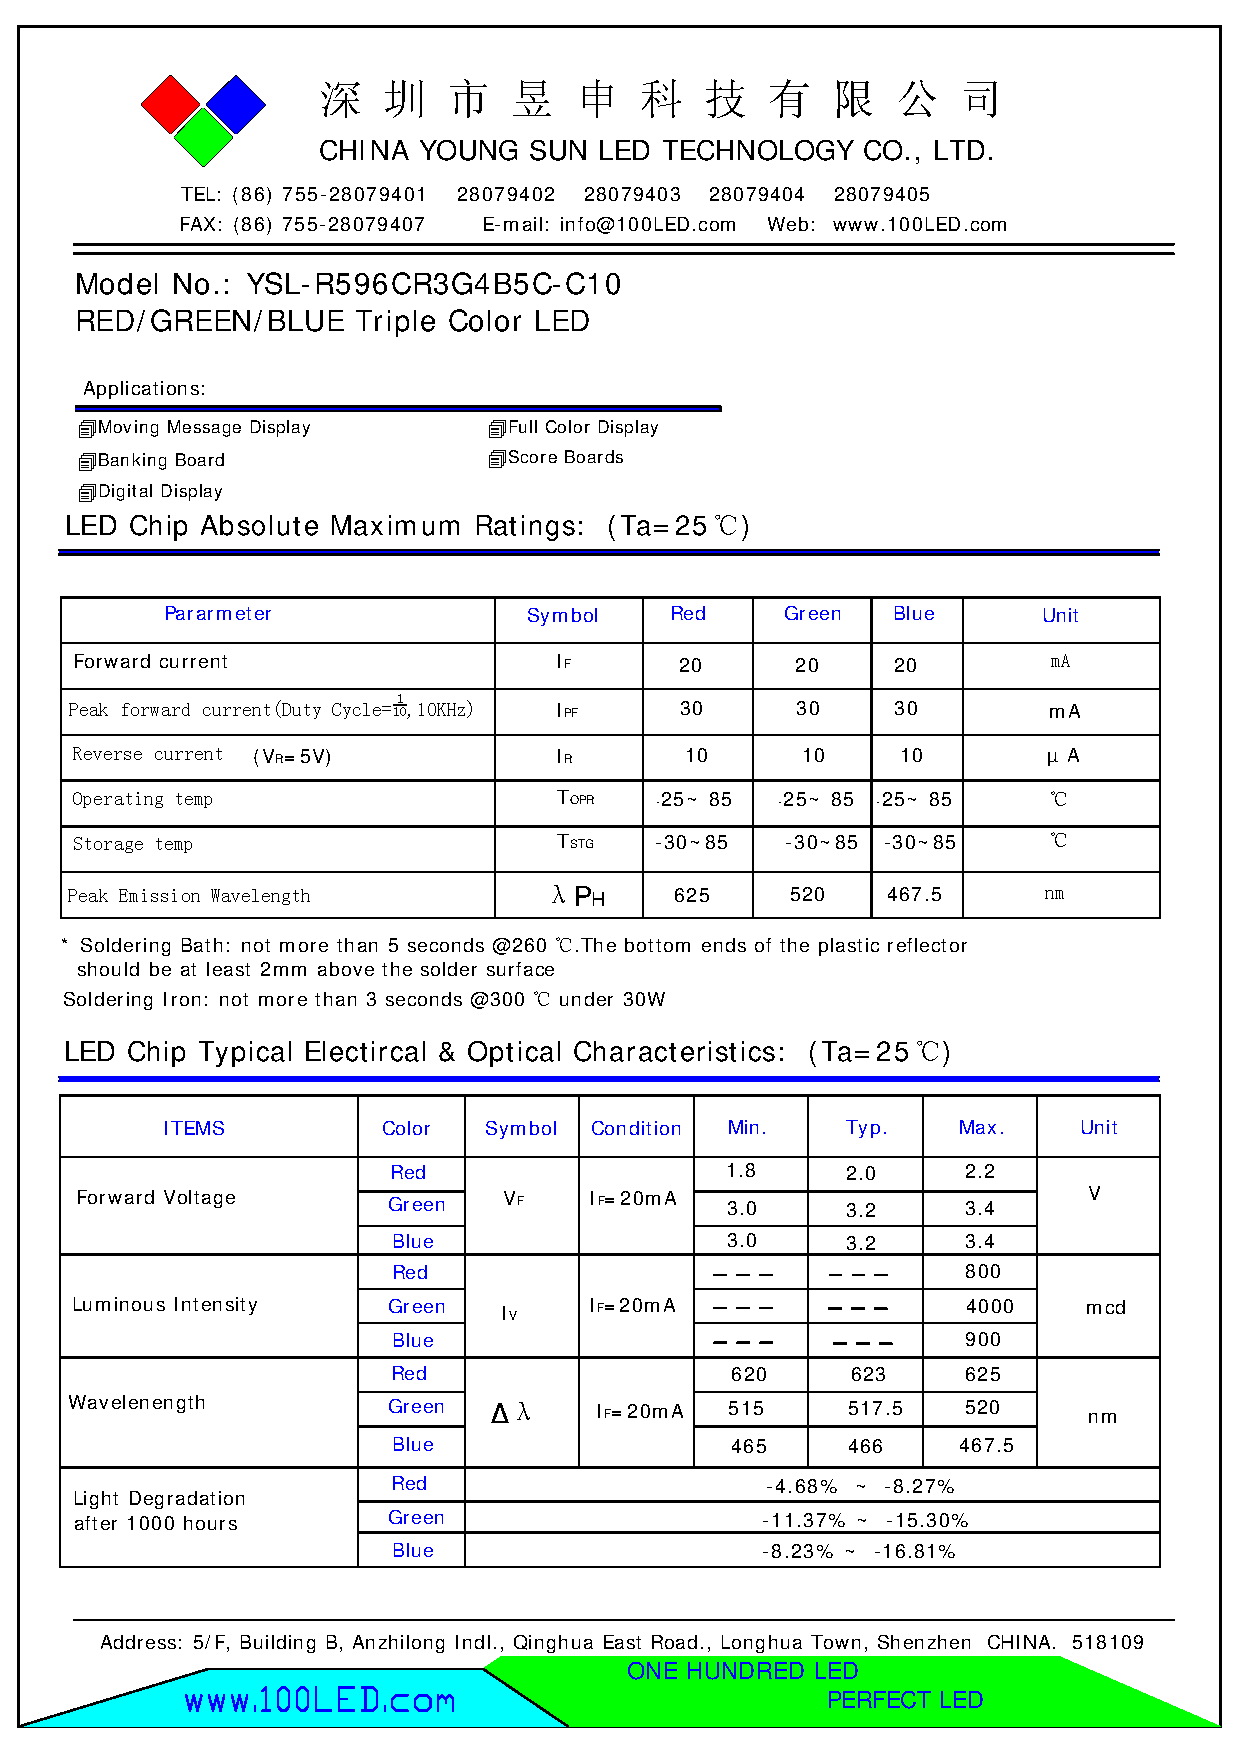
\includepdf[pages={1-3}]{Documentos/LED.pdf} 
  
  

\end{document}
 